\documentclass[11pt,a4paper]{report}
\usepackage[greek,english]{babel}
\title{{Aristotle University of Thessaloniki\\Group Project for the Game Theory Course\\ Group 01\\[2em]\textbf{Imitation and Fitness Dynamics on Iterated Prisoner's Dilemma}}\\}
\usepackage{titlepic}
\usepackage[dvipsnames]{xcolor}
%\usepackage[lite]{mtpro2}
%\usepackage{mathptmx} 
%\usepackage{newtxtext}
\usepackage{tcolorbox}
\usepackage{multirow}
\author{Ιωάννης Λαζαρίδης\\10431\\\texttt{ilazarit@ece.auth.gr} \and Κωνσταντίνος Βλαχάκος\\10403\\\texttt{kvlachak@ece.auth.gr} \and Ιωάννης Κοσμάς Βαρδάκης\\10498\\ \texttt{ivardakis@ece.auth.gr}}
\titlepic{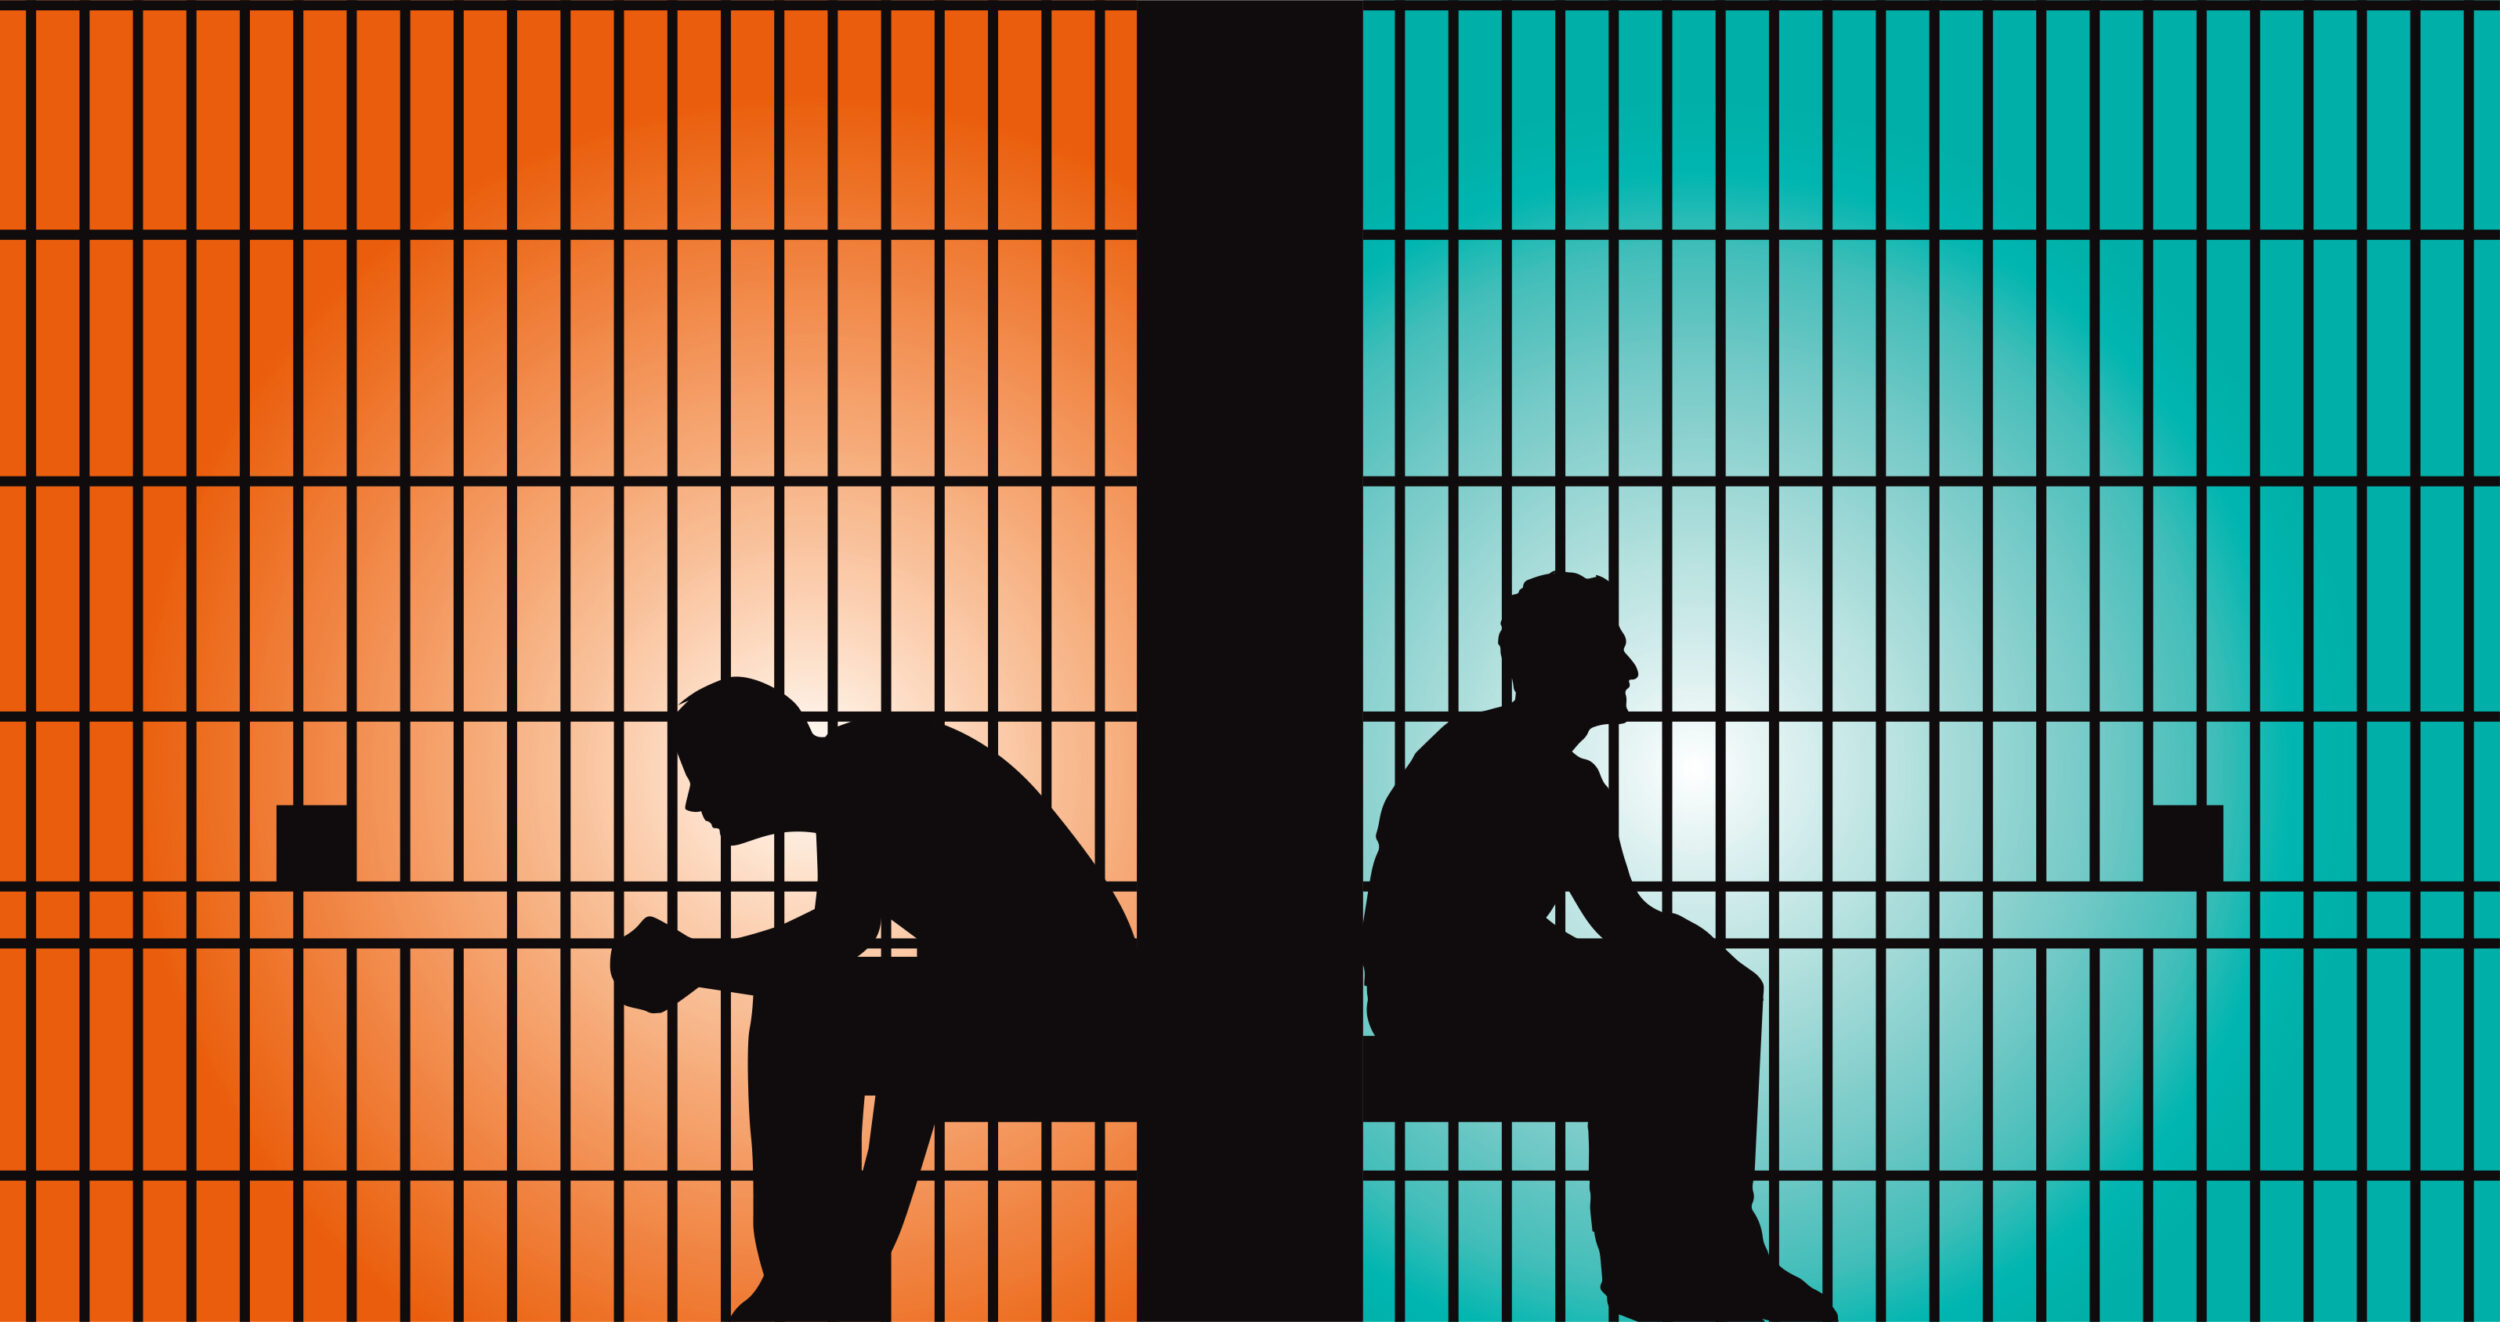
\includegraphics[width=\textwidth]{ela.png}}
%\usepackage{fontspec}
%\usepackage[utf8]{inputenc}
\usepackage{indentfirst}
%\usepackage{kerkis}
\usepackage[T1]{fontenc}
\setcounter{section}{0}
\date{May 2025}
%\setmainfont[BoldFont=Times New Roman Greek Bold,ItalicFont=Times New Roman Greek Inclined]  {Times New Roman Greek}
\renewcommand{\cite}[1]{[\ref{#1}]}
%\usepackage{newtxmath}
\usepackage{amssymb}
\usepackage{amsthm}
%\usepackage{mtpro2}
\usepackage[greek,english]{babel}
\usepackage{alphabeta}
\usepackage{bigints}
\usepackage[toc,page]{appendix}
\usepackage{bm}\def\mathclap#1{\text{\hbox to 0pt{\hss$\mathsurround=0pt#1$\hss}}}
\newtcolorbox{mybox}{colback=white!80!yellow,colframe=black!65!white}
\newtcolorbox{box1}{colback=white!75!Red,colframe=black!85!white}
%\newtcolorbox{mybox}{colback=white!80!yellow,colframe=black!65!white}
\newcommand{\dd}[2]{\frac{d #1}{d#2}}
%\newfontfamily{\trb}{Times New Roman Greek Bold}
%\newenvironment{tnrb}{\trb}{\par}
\usepackage{fontawesome5}
\usepackage{etoolbox}
\thinmuskip=5mu    % Default: 3mu (affects \, and automatic thin spaces)
\medmuskip=5mu     % Default: 4mu (affects \: and operators like +, -)
\thickmuskip7mu
\usepackage{cancel}
\usepackage{geometry}
\geometry{
	a4paper,
	total={170mm,257mm},
	left=20mm,
	top=20mm,
}
\usepackage{hyperref}
\renewcommand{\d}{\,\mathrm{d}}
\renewcommand{\a}{\mathcal{A}}
\newcommand{\z}{\frac{1}{2\pi}}
\newcommand{\norm}[1]{\lVert #1 \rVert_1}
\newcommand{\pnorm}[2]{\lVert #1 \rVert_#2}
\newcommand{\s}{\sin}
\renewcommand{\c}{\cos}
\renewcommand{\qed}{\hfill \(\blacksquare\)}
\newcommand{\fc}{e^{-inx}}
\newcommand{\sn}{\sum_{k=-N}^{N}}
\usepackage{listings}
\usepackage{xcolor}

\definecolor{codegreen}{rgb}{0,0.6,0}
\definecolor{codegray}{rgb}{0.5,0.5,0.5}
\definecolor{codepurple}{rgb}{0.58,0,0.82}
\definecolor{backcolour}{rgb}{0.95,0.95,0.92}

\lstdefinestyle{mystyle}{
	backgroundcolor=\color{backcolour},   
	commentstyle=\color{codegreen},
	keywordstyle=\color{magenta},
	numberstyle=\tiny\color{codegray},
	stringstyle=\color{codepurple},
	basicstyle=\ttfamily\footnotesize,
	breakatwhitespace=false,         
	breaklines=true,                 
	captionpos=b,                    
	keepspaces=true,                 
	numbers=left,                    
	numbersep=5pt,                  
	showspaces=false,                
	showstringspaces=false,
	showtabs=false,                  
	tabsize=2,
	language=Matlab
}

\lstset{style=mystyle}
\AtBeginEnvironment{lstlisting}{\vspace{1em}}
\AtEndEnvironment{lstlisting}{\vspace{1em}}
\usepackage{fancyhdr}

\pagestyle{fancy}
\fancyhf{}
%\fancyhead[L]{\leftmark} % Chapter/section info
%\fancyhead[R]{\thepage} % Page number on right

\makeatletter
\renewcommand{\@chapapp}{Κεφάλαιο}  % This replaces "Chapter" with "Part"
\makeatother
\usepackage{nameref}
\begin{document}

	\maketitle{}
	\tableofcontents
\setcounter{chapter}{-1}
\chapter{Εισαγωγή}
Η παρούσα εργασία πραγματεύεται την υλοποίηση του εξελικτικού πρωταθλήματος \textit{Axelrod}, το οποίο έχει ως θεωρητική βάση το επαναλαμβανόμενο δίλημμα του φυλακισμένου (Iterated Prisoner's Dilemma - IPD). Η εργασία αυτή αποτελεί το πέμπτο παραδοτέο στο πλαίσιο του μαθήματος της Θεωρίας Παιγνίων, και ακολουθεί προηγούμενες εργασίες στις οποίες έχουν υλοποιηθεί:(α) το περιβάλλον του παιχνιδιού,(β) οι βασικές στρατηγικές που χρησιμοποιούνται στα πειράματα.
Για την καλύτερη κατανόηση, είναι σημαντικό να εξηγηθεί πρώτα τι είναι το δίλημμα του φυλακισμένου και το πρωτάθλημα Axelrod.

\subsubsection*{Το Δίλημμα του Φυλακισμένου}
Το κλασικό δίλημμα του φυλακισμένου είναι ένα υποθετικό σενάριο συνεργασίας και προδοσίας μεταξύ δύο παικτών. Κάθε παίκτης έχει δύο επιλογές: να συνεργαστεί (\textbf{C}) ή να προδώσει (\textbf{D}). Οι αποδόσεις (\textbf{payoffs}) κάθε παίκτη εξαρτώνται από τον συνδυασμό των επιλογών τους και μπορούν να περιγραφούν με τέσσερις βασικές τιμές:
\begin{itemize}
	\item \textbf{T (Temptation to Defect)} η ανταμοιβή που παίρνει κάποιος όταν προδίδει ενώ ο άλλος συνεργάζεται.
	\\
	\item \textbf{R (Reward for Mutual Cooperation)}: η ανταμοιβή που παίρνουν και οι δύο όταν συνεργάζονται.
	\\
	\item \textbf{P (Punishment for Mutual Defection)}: η τιμωρία που λαμβάνουν όταν και οι δύο προδίδουν.
	\\
	\item 
	\textbf{S (Sucker's Payoff)}: η "ζημιά" που υφίσταται κάποιος όταν συνεργάζεται ενώ ο άλλος τον προδίδει
	
\end{itemize}
Ο πίνακας αποδόσεων (\textit{payoff matrix}) έχει ως εξής:
\begin{table}[h]
	\centering
	
	\vspace*{2em}
	\begin{tabular}{cc|c|c|}
		& \multicolumn{1}{c}{} & \multicolumn{2}{c}{P2} \\
		& \multicolumn{1}{c}{} & \multicolumn{1}{c}{C (Συνεργασία)} & \multicolumn{1}{c}{D (Προδοσία)} \\\cline{3-4}
		\multirow{2}*{P1} & C & R, R & S, T \\\cline{3-4}
		& D & T, S & P, P \\\cline{3-4}
	\end{tabular}
	\caption{Payoff Matrix}
\end{table}\\
Οι τυπικές τιμές που χρησιμοποιούνται στο IPD είναι:
\(T = 5, R = 3, P = 1, S = 0\)
\\
\clearpage
Για να υπάρχει πραγματικό «δίλημμα», πρέπει να ισχύουν δύο βασικές \textbf{λογικές συνθήκες:
}
\begin{enumerate}
	\item \(\bm{S<P<R<T}\)\\
	Δηλαδή: είναι χειρότερο να σε προδώσουν ενώ συνεργάζεσαι \((S)\), από το να προδώσετε και οι δύο \((P)\), και προτιμότερο να συνεργαστείτε και οι δύο \((R)\), αλλά ο μεγαλύτερος πειρασμός είναι να προδώσεις όταν ο άλλος συνεργάζεται \((T)\).
	\\
	\item \(\bm{S + T < 2R}\) \\Αυτή η επιπλέον συνθήκη εξασφαλίζει ότι η\textbf{ συνεργασία είναι συλλογικά προτιμότερη} από την εναλλαγή μεταξύ προδοσίας και συνεργασίας. Δηλαδή, αν οι παίκτες εναλλάσσονται μεταξύ \(C \) και \(D\), οι αποδόσεις είναι χειρότερες από τη σταθερή συνεργασία.
	\\
	\\
	Το δίλημμα έγκειται στο γεγονός ότι, ενώ η \textbf{αμοιβαία συνεργασία} οδηγεί σε καλύτερη συνολική απόδοση και για τους δύο \((R)\), η \textbf{προδοσία είναι η ατομικά καλύτερη επιλογή}, ανεξάρτητα από την κίνηση του άλλου. Αυτό συμβαίνει επειδή:
	\begin{itemize}
		\item Αν ο άλλος συνεργάσει, το να προδώσεις σου δίνει \(\bm{T > R}\)
		\item Αν ο άλλος προδώσει, το να προδώσεις σου δίνει \(\bm{P > S}\)
		
		
	\end{itemize}
	Έτσι, η προδοσία είναι \textbf{το μοναδικό σημείο ισορροπίας Nash} στο παίγνιο μίας φοράς. Ωστόσο, όπως θα δούμε στη συνέχεια, όταν το παιχνίδι επαναλαμβάνεται, μπορούν να προκύψουν πολύ διαφορετικές δυναμικές.
	
\end{enumerate}
\subsection*{Επαναλαμβανόμενο Δίλημμα του Φυλακισμένου (IPD)}
Επαναλαμβανόμενο Δίλημμα του Φυλακισμένου (Iterated Prisoner's Dilemma)

Σε αντίθεση με το απλό παίγνιο που παίζεται μόνο μία φορά, \textbf{στο επαναλαμβανόμενο δίλημμα του φυλακισμένου}, οι δύο παίκτες παίζουν πολλές φορές μεταξύ τους, και μπορούν να βασίσουν την απόφασή τους για την επόμενη κίνηση στις προηγούμενες κινήσεις του αντιπάλου. Αυτό επιτρέπει την εμφάνιση πιο πολύπλοκων στρατηγικών, όπως η \textbf{Tit for Tat} (ξεκινά με συνεργασία και έπειτα αντιγράφει την προηγούμενη κίνηση του αντιπάλου), και δημιουργεί δυναμική αλληλεπίδρασης και «μνήμης».

\subsection*{Το Πρωτάθλημα Axelrod}
Το \textbf{Πρωτάθλημα Axelrod} ήταν ένα διάσημο υπολογιστικό πείραμα που διεξήγαγε ο πολιτικός επιστήμονας \textbf{Robert Axelrod} τη δεκαετία του 1980. Ο Axelrod προσκάλεσε ερευνητές να υποβάλουν στρατηγικές για το επαναλαμβανόμενο δίλημμα του φυλακισμένου. Οι στρατηγικές αυτές διαγωνίστηκαν μεταξύ τους σε ένα τουρνουά όπου η κάθε στρατηγική έπαιζε επαναλαμβανόμενα παιχνίδια με όλες τις υπόλοιπες, συγκεντρώνοντας βαθμούς με βάση τα αποτελέσματα κάθε αναμέτρησης.
Το τουρνουά του Axelrod ανέδειξε τη σημασία της συνεργασίας και της «τιμωρίας με μέτρο» ως αποτελεσματική στρατηγική. Χαρακτηριστικά, η απλή στρατηγική \textbf{Tit for Tat} αναδείχθηκε ως μία από τις πιο επιτυχημένες, αναδεικνύοντας τη δύναμη της αμοιβαιότητας στη σταθερή συνεργασία.
\clearpage
\subsection*{Σκοπός και Δομή της Παρούσας Εργασίας
}Η εργασία επικεντρώνεται στην \textbf{εξελικτική εκδοχή} του τουρνουά, όπου οι στρατηγικές «επιβιώνουν» ή «αντικαθίστανται» ανάλογα με την απόδοσή τους. Αναλυτικότερα, η εργασία χωρίζεται σε δύο βασικές προσεγγίσεις
\begin{enumerate}
	\item \textbf{Imitation Dynamics}\\ Σε αυτό το μοντέλο, σε κάθε γενιά ένας αριθμός παικτών αντικαθιστά τη στρατηγική του με εκείνη κάποιου άλλου που έχει καλύτερη απόδοση (Score). Ο πληθυσμός εξελίσσεται μιμούμενος τις καλύτερες στρατηγικές.
	\item 	\textbf{Fitness Dynamics}: Σε αυτή την προσέγγιση, η πιθανότητα να επιβιώσει ή να αναπαραχθεί μια στρατηγική εξαρτάται από το μέσο Score που συγκεντρώνει. Πρόκειται για πιο αναλυτική, συνεχής προσέγγιση εμπνευσμένη από τη βιολογική εξέλιξη.
	
\end{enumerate}
Η βασική διαφορά μεταξύ των δύο μοντέλων έγκειται στον τρόπο που οι στρατηγικές διαδίδονται στον πληθυσμό:
\begin{itemize}
	\item Στο \textbf{Fitness Dynamics}, η αλλαγή εξαρτάται από το \textbf{συνολικό αποτέλεσμα} κάθε στρατηγικής σε κάθε γενιά.
	\item Στο \textbf{Imitation Dynamics}, επικεντρωνόμαστε στους \textbf{καλύτερους παίκτες}, και οι αλλαγές είναι διακριτές και συμβαίνουν σε \textbf{συγκεκριμένο αριθμό} παικτών ανά γενιά.
	
\end{itemize}Στη θεωρητική ανάλυση του Fitness Dynamics, επιβεβαιώνονται τα αποτελέσματα των \cite{paper} Mathieu et al., ενώ στο Imitation Dynamics γίνεται υλοποίηση της \textbf{αλυσίδας Markov} για όλες τις πιθανές κατανομές πληθυσμού, ανάλογα με το μέγεθος πληθυσμού και τη δυναμική μετάβασης.

\chapter{Quickstart}
Τα αρχεία μας βρίσκονται στο παρακάτω \href{https://github.com/vasilomanitaros/EvolutionaryGamesToolbox}{github repo} : για την κλήση οποιουδήποτε πειράματος χρησιμοποιούμε το script \texttt{base.m } με την οποία ο χρήστης μπορεί να αναπαραγάγει τα πειράματα που έχουμε κάνει και εμείς. Σε γενικότερο πλαίσιο, ο κώδικάς μας αναπαράγει τα αποτελέσματα από το paper\cite{paper}
αλλα και να κάνει πειράματα προσομοίωσης πάνω σε αυτό. Επιπλέον μπορεί να αναπαράξει τόσο αποτελέσματα θεωρητικής ανάλυσης, τόσο και αποτελέσματα Imitation, όπως αναλύσαμε στο μάθημα. Οι βασικές συναρτήσεις που υλοποιούν τους αλγορίθμους με τους οποίους γίνονται αυτές οι διαδικασίες είναι οι: \texttt{TourTheFit}, \texttt{TourTheFit2}, \texttt{TourSimFit}, \texttt{TourTheImi}, \texttt{TourTheImi2},
\texttt{TourSimImi}. 
\par 
Για το repository δεν απαιτείται κάποια ειδική εγκατάσταση πέραν του απλού \texttt{git clone} καθώς όλα τα paths των scripts είναι relative. Σε περίπτωση απροοπτου προβλήματος μπορείτε να επικοινωνήσετε μαζί μας στα παραπάνω email.
\chapter{Fitness Dynamics}
\section{Θεωρητική Ανάλυση του Fitness Dynamics}
Σε αυτό το σημείο θα αναλύσουμε την  \nameref{appendix:TourTF} .



Τα ορίσματα όπως ζητάει η εκφώνηση είναι το B ο πίνακας του παίγνιου, το Strategies που είναι διάνυσμα \texttt{strings} με τις στρατηγικές και συμπληρώνεται από το \texttt{Pop0} το οποίο είναι ο αρχικός πλυθησμός που παρευρίσκεται στο παιχνίδι. Το \( Τ\) ο αριθμός των γύρων και το \(J\) ο αριθμός των γενεών που θα τρέχει το πρωτάθλημα.
Αρχικά λαμβάνουμε τον πίνακα \texttt{Re\_matrix} (από τη συνάρτηση \nameref{appendix:RewST} ) ο οποίος είναι ο πίνακας των Scores μετά από έναν συγκεκριμένο αριθμό γύρων. 
\\

Η συνάρτηση αυτή υλοποιεί ένα παιχνίδι Axel \(Τ\) γύρων και επιστρέφει τον πίνακα με τα scores μεταξύ των στρατηγικών. 
Στη συνέχεια, λαμβάνουμε στην μεταβλητή \(P\) το άθροισμα των πληθυσμών στις στρατηγικές που παίζουμε δηλαδή τον αρχικό συνολικό πληθυσμό και αρχικοποιούμε τις μεταβλητές επιστροφής.
\\

 To \texttt{POP} επιστρέφει τις τιμές του πληθυσμού ανά γενιά, το \texttt{BST} τις βέλτιστες στρατηγικές ανα γενιά ενώ το \texttt{FIT} το fitness των στρατηγικών. Στη συνέχεια αναθέτουμε τον αρχικό πληθυσμό στην πρώτη θέση του array του \texttt{POP} και υπολογίζουμε το fitness της κάθε στρατηγικής δηλαδή το άθροισμα των score επί τον πλυθησμό με βάση τη συγκεκριμένη στρατηγική αφαιρώντας τις περιπτώσεις που οι στρατηγικές παίζουν με τον εαυτό τους όπως αναλύεται και στο paper\cite{paper}.
\\

Στη συνέχεια υπολογίζονται οι συνολικοί πόντοι \(t\) που έχουν δοθεί σε όλες τις στρατηγικές και ψάχνουμε να βρούμε αυτές με το βέλτιστο fitness για την έξοδο του \texttt{BST}.
\\
Ο πληθυσμός ανανεώνεται με βάση τους τύπους του paper\cite{paper}: \begin{align*}
W_{n+1}(A) &= \frac{\Pi W_n(A) g_n(A)}{t(n)} \\
W_{n+1}(B) &= \frac{\Pi W_n(B) g_n(B)}{t(n)} \\
W_{n+1}(C) &= \frac{\Pi W_n(C) g_n(C)}{t(n)}
\end{align*} και το ερώτημα που γεννάται είναι κατά πόσο η ανάλυση αυτή είναι σωστή με την παραδοχή ότι δεν γίνεται στρογγυλοποίηση και το \texttt{POP} διάνυσμα περιέχει πραγματικές τιμές.
Για τον σκοπό αυτό προσθέτουμε την προτροπή του paper σύμφωνα με το οποίο οι πληθυσμοί της επόμενης γενιάς υπλογίζονται από το floor της κάθε παράστασης.
Εδώ πέρα γεννάται το ερώτημα εάν το συγκεκριμένο «επιπόλαιο» rounding κρατήσει ίδιο τον συνολικό πληθυσμό και με την πρώτη δοκιμή παρατηρούμε ότι δεν τον κρατάει. Συνεπώς πρέπει να αποφασίσουμε αν θα χρησιμοποιήσουμε τον ίδιο πληθυσμό με τον αρχικό ή κάθε φορά θα τον ξαναμετράμε για να συμπεριλάβουμε το σφάλμα του rounding. Ωστόσο στη δεύτερη περίπτωση παρατηρούμε το σφάλμα ανά γενιά να συσσωρεύεται οδηγώντας στην κατάρρευση του συστήματος. 
Συνεπώς η υλοποίηση η οποία ακολουθεί πιστά και το paper είναι να μετρήσουμε μια φορά τον συνολικό πληθυσμό και σε κάθε γενιά να χρησιμοποιούμε αυτή τη σταθερή τιμή \(P \) κάνοντας floor rounding ακόμα και αν αυτό οδηγήσει στο τέλος σε μια μικρή απώλεια.
Τα αποτελέσματα που παρήχθησαν μπορούν να φανούν παρακάτω:
\begin{figure}[htbp]
\vspace*{1em}
  \centering
  \begin{minipage}{0.48\textwidth}
    \centering
 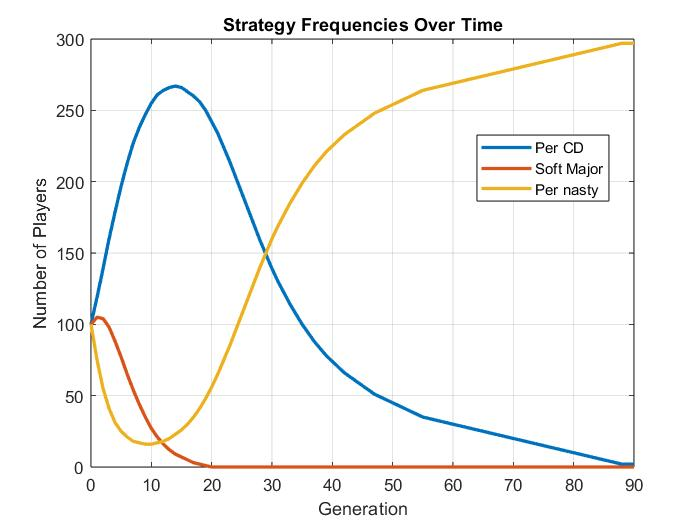
\includegraphics[width=0.8\linewidth]{fit_plots_theoretical/defectors_may_be_strong}

\label{fig:defectorsmaybestrong}
  \end{minipage}
  \hfill
  \begin{minipage}{0.48\textwidth}
    \centering
  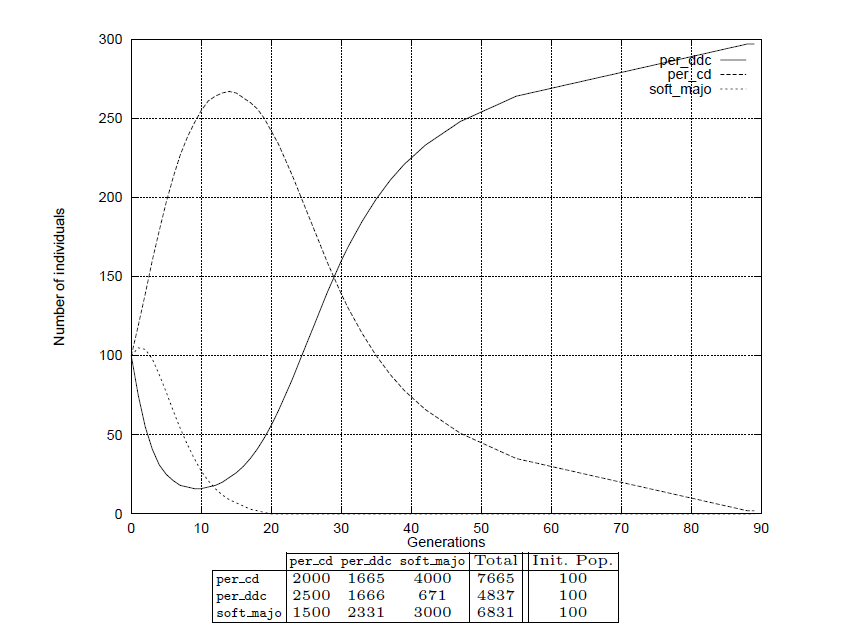
\includegraphics[width=0.8\linewidth]{defectors_may_be_strong }

  \end{minipage}
  \caption{Defectors may be Strong (\texttt{defectors\_may\_be\_strong.m})}
\end{figure}

\begin{figure}[htbp]
  \centering
  \begin{minipage}{0.48\textwidth}
    \centering
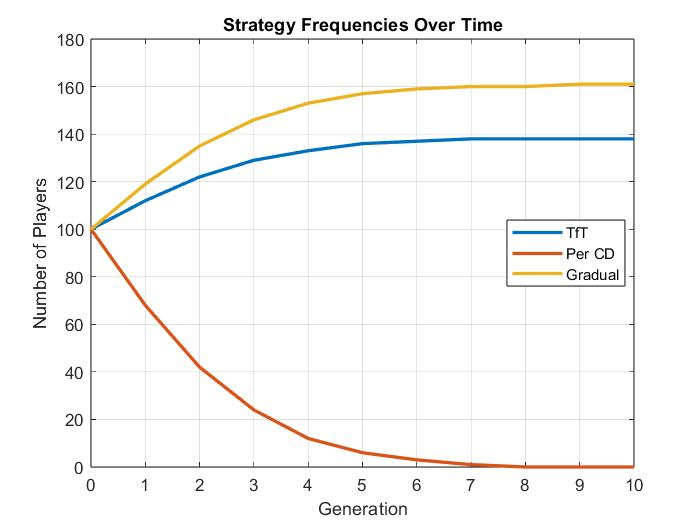
\includegraphics[width=0.8\linewidth]{fit_plots_theoretical/monotonous_convergence}

  \end{minipage}
  \hfill
  \begin{minipage}{0.48\textwidth}
    \centering
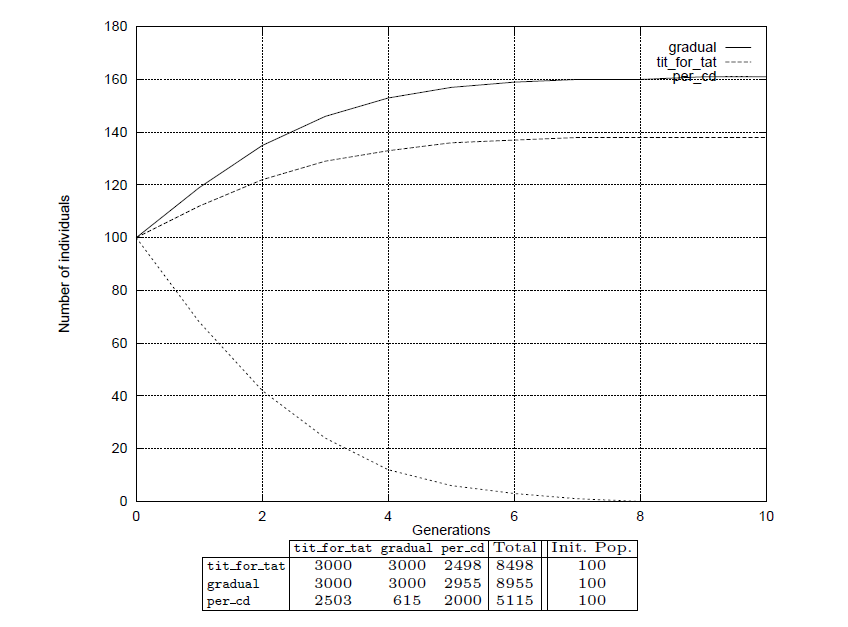
\includegraphics[width=0.8\linewidth]{monotonous_convergence}

  \end{minipage}\caption{Monotonous Convergence (\texttt{monotonous\_convergence.m})}
\end{figure}

\begin{figure}[htbp]
	\centering
	\begin{minipage}{0.48\textwidth}
		\centering
		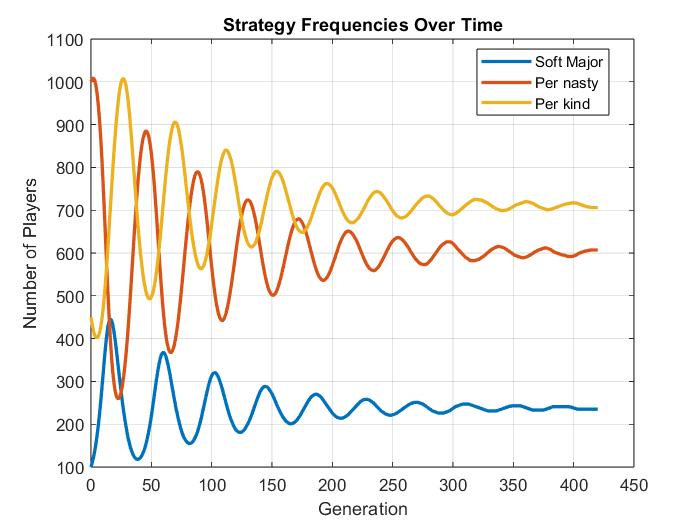
\includegraphics[width=0.8\linewidth]{fit_plots_theoretical/attenuated_oscillatory_movements}
	
	\end{minipage}
	\hfill
	\begin{minipage}{0.48\textwidth}
		\centering
		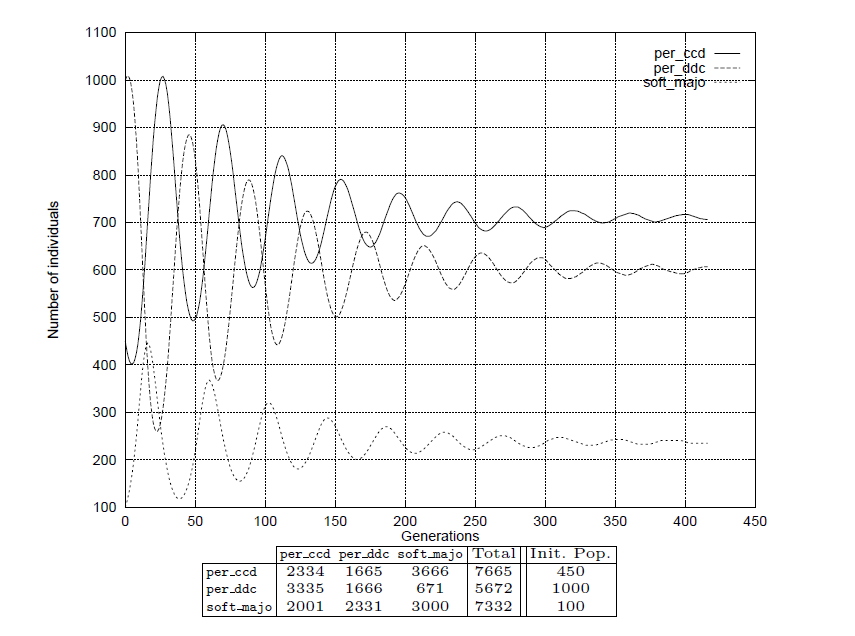
\includegraphics[width=0.8\linewidth]{attenuated_oscillatory_movements}
	
	\end{minipage}
		\caption{Attenuated\_oscillatory\_movements (\texttt{attenuated\_oscillatory\_movements.m})}

\end{figure}
\clearpage





% TODO: \usepackage{graphicx} required
\begin{figure}[ht!]
\centering
	\begin{minipage}{0.48\textwidth}
	\includegraphics[width=1\linewidth]{fit_plots_theoretical/Increasing_Oscillations}

	
	\end{minipage}
	\begin{minipage}{0.48\textwidth}
		\includegraphics[width=1\linewidth]{Increasing_Oscillations}
	\end{minipage}
	\caption{Increasing Oscillations (\texttt{increasing\_oscillations.m})}
\end{figure}

\begin{figure}[ht!]
	\centering
	\begin{minipage}{0.48\textwidth}
		\includegraphics[width=1\linewidth]{fit_plots_theoretical/Periodic_Movements}
		
		
	\end{minipage}
	\begin{minipage}{0.48\textwidth}
		\includegraphics[width=1\linewidth]{Periodic_Movements}
	\end{minipage}
	\caption{Periodic Movements \texttt{(periodic\_movements.m)}}
\end{figure}

\begin{figure}[ht!]
	\centering
	\begin{minipage}{0.48\textwidth}
		\includegraphics[width=1\linewidth]{fit_plots_theoretical/Disordered_Oscillations}
		
		
	\end{minipage}
	\begin{minipage}{0.48\textwidth}
		\includegraphics[width=1\linewidth]{Disordered_Oscillations}
	\end{minipage}
	\caption{Disordered Oscillations \texttt{(Disordered Oscillations.m)}}
\end{figure}

\begin{figure}[ht!]
	\centering
	\begin{minipage}{1\textwidth}
		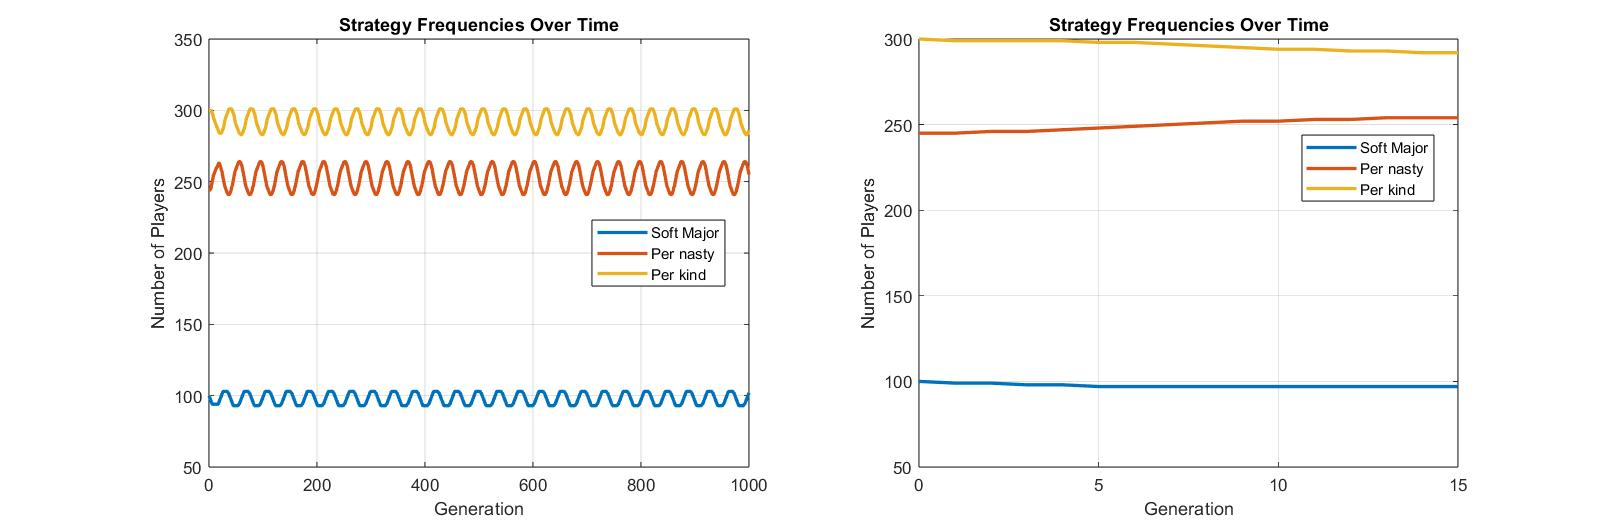
\includegraphics[width=1\linewidth]{fit_plots_theoretical/sensitivity_to_population_size}
		
		
	\end{minipage}
	\begin{minipage}{1\textwidth}
		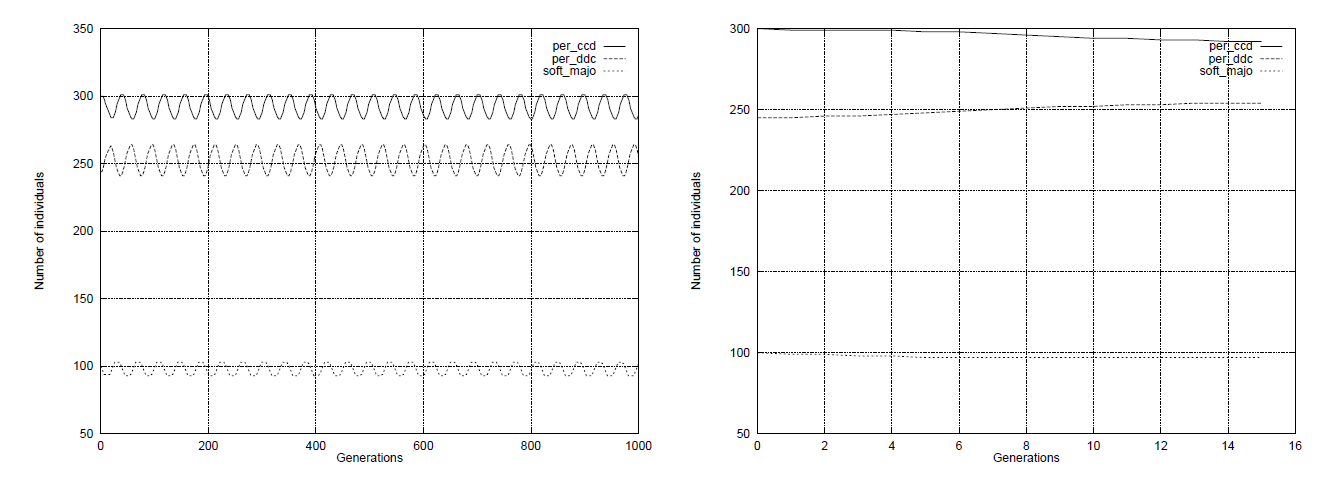
\includegraphics[width=1\linewidth]{sens_popsize}
	\end{minipage}
	\caption{Sensitivity of dynamics to population's size. All parameters are identical except
		for the initial size of per ddc which is 244 on the left and 245 on the right \texttt{(sens\_dyn\_pop\_size.m)}}
\end{figure}

\begin{figure}[ht!]
	\centering
	\begin{minipage}{1\textwidth}
		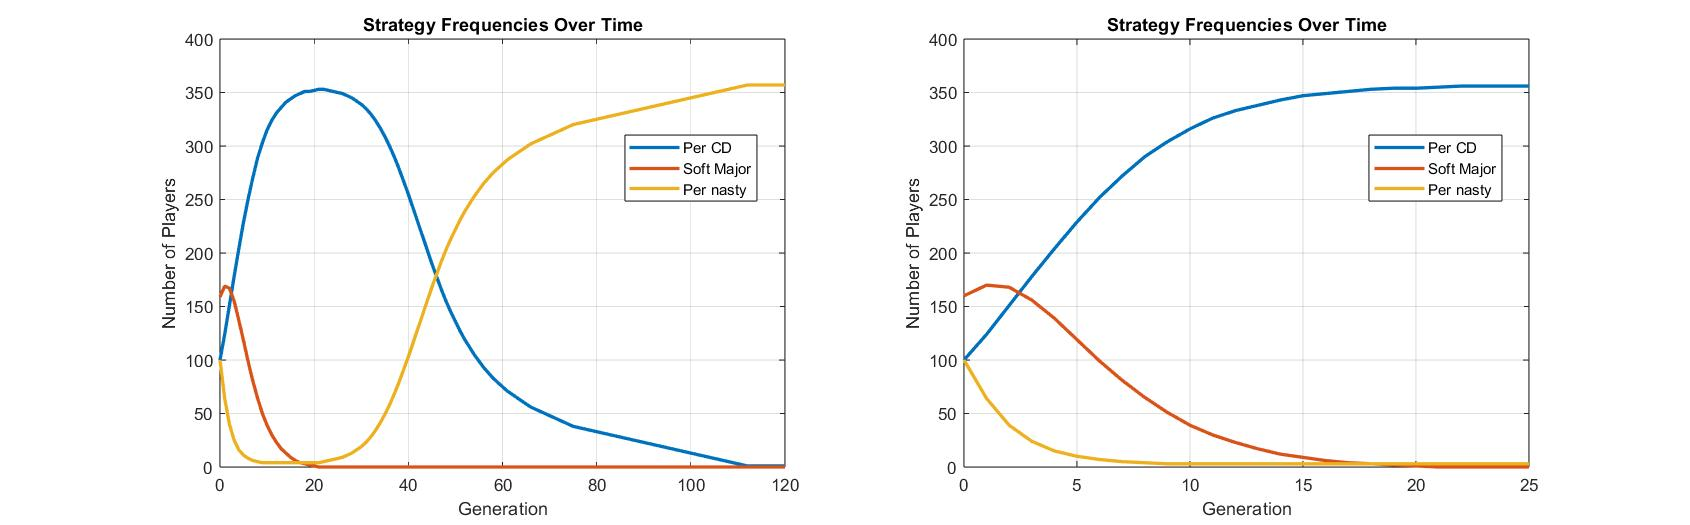
\includegraphics[width=1\linewidth]{fit_plots_theoretical/sensitivity_of_winner_to_popsize}
		
		
	\end{minipage}
	\begin{minipage}{1\textwidth}
		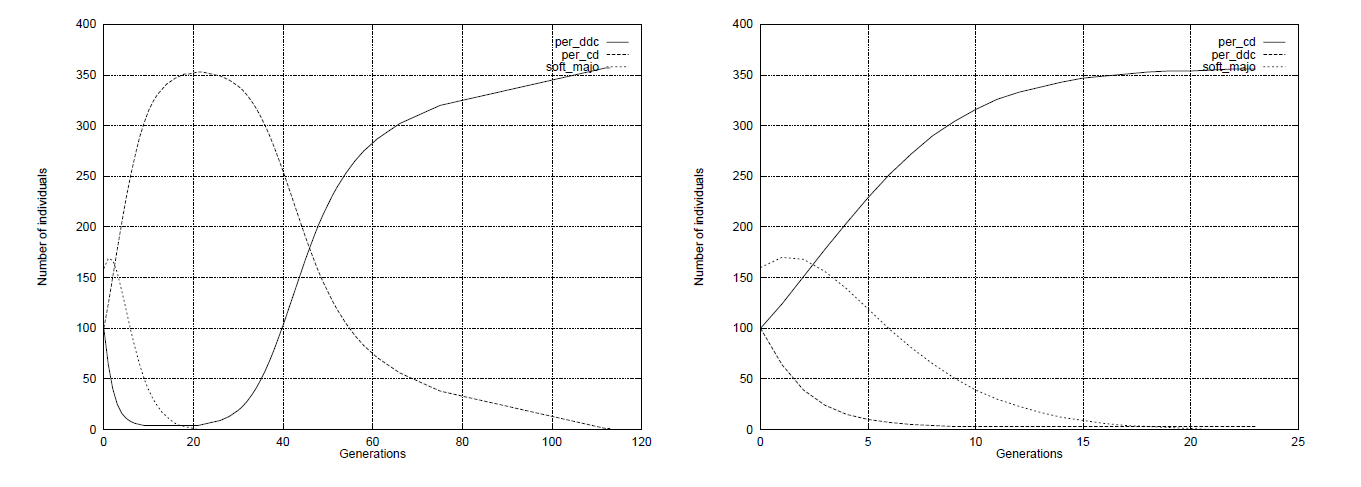
\includegraphics[width=1\linewidth]{sens_winner}
	\end{minipage}
	\caption{Sensitivity of winner to population's size. All parameters are identical except
		for the initial size of soft majo which is 159 on the left and 160 on the right.(\texttt{sens\_win\_pop\_size.m})}
\end{figure}

\begin{figure}[ht!]
	\centering
	\begin{minipage}{1\textwidth}
		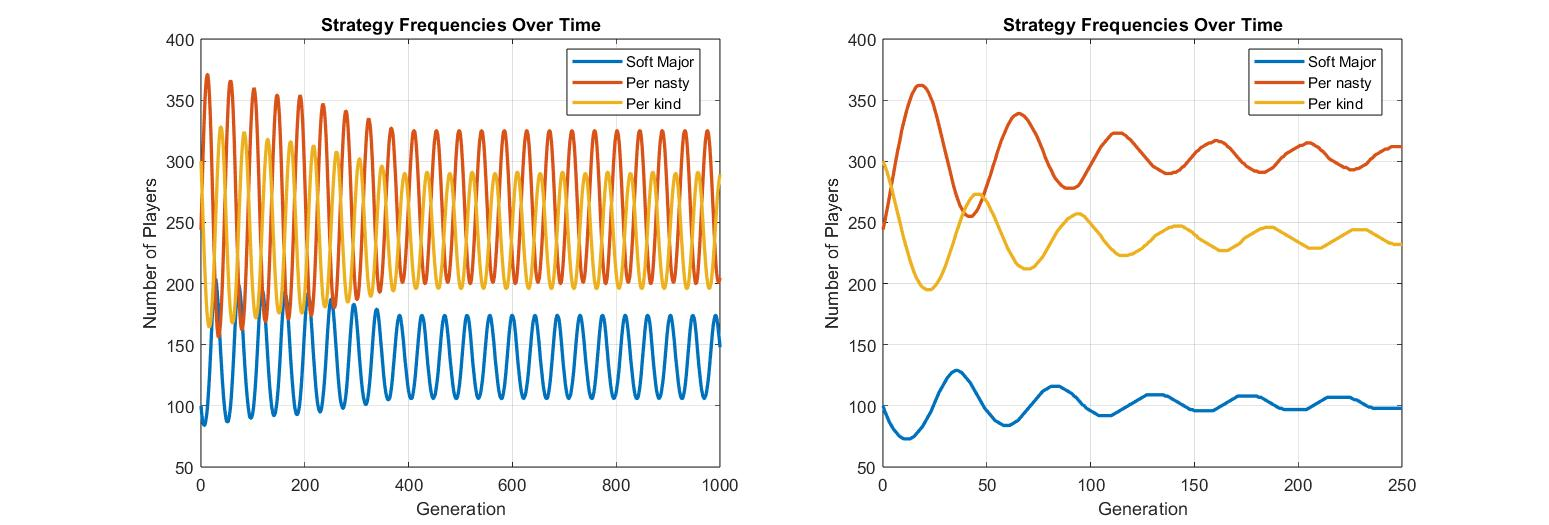
\includegraphics[width=1\linewidth]{fit_plots_theoretical/sensitivity_to_game_length}
		
		
	\end{minipage}
	\begin{minipage}{1\textwidth}
		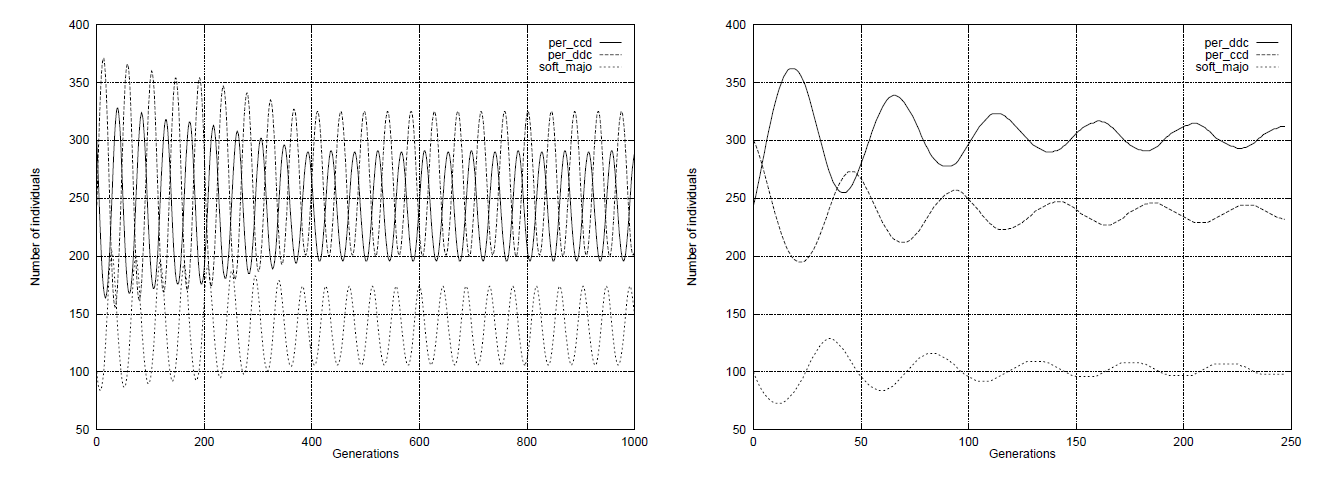
\includegraphics[width=1\linewidth]{sens_gamelength}
	\end{minipage}
	\caption{Sensitivity to game length. All parameters are identical except for the game
	length which is 7 moves on the left and 6 on the right \texttt{(sens\_game\_length.m)}}
\end{figure}


\begin{figure}[ht!]
	\centering
	\begin{minipage}{1\textwidth}
		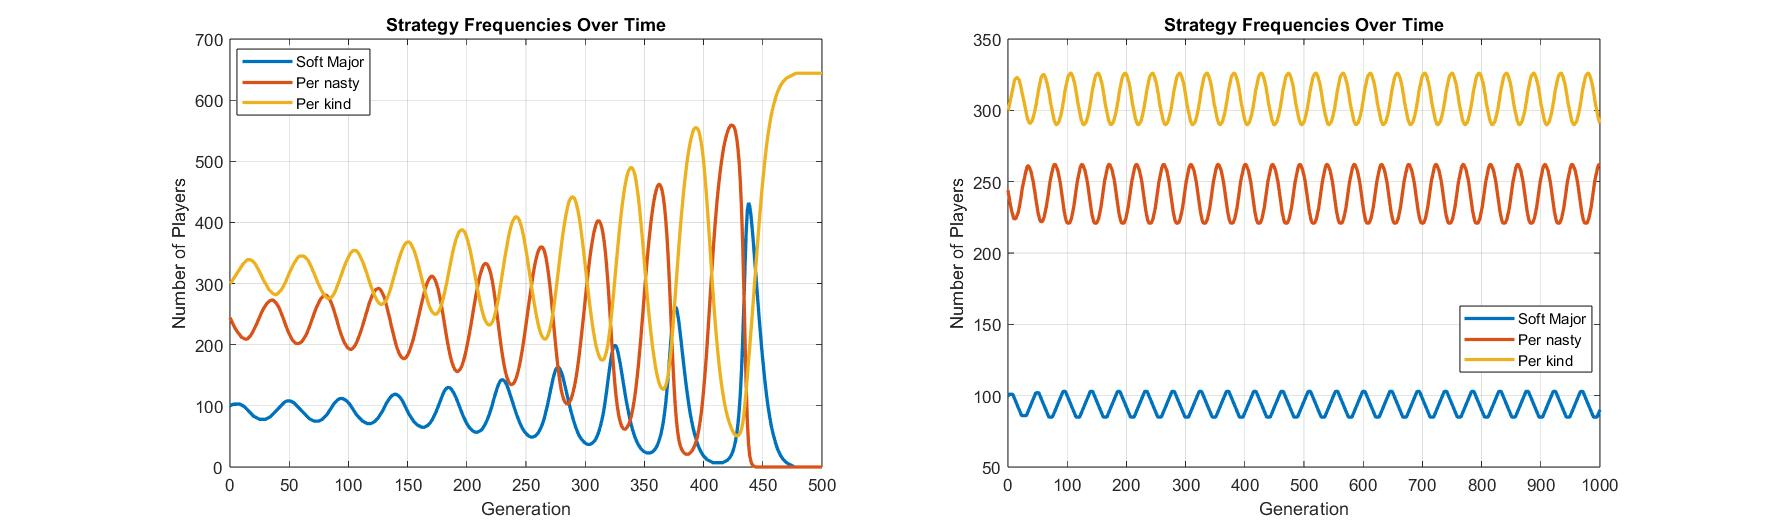
\includegraphics[width=1\linewidth]{fit_plots_theoretical/sensitivity_to_cipd_payoff}
		
		
	\end{minipage}
	\begin{minipage}{1\textwidth}
		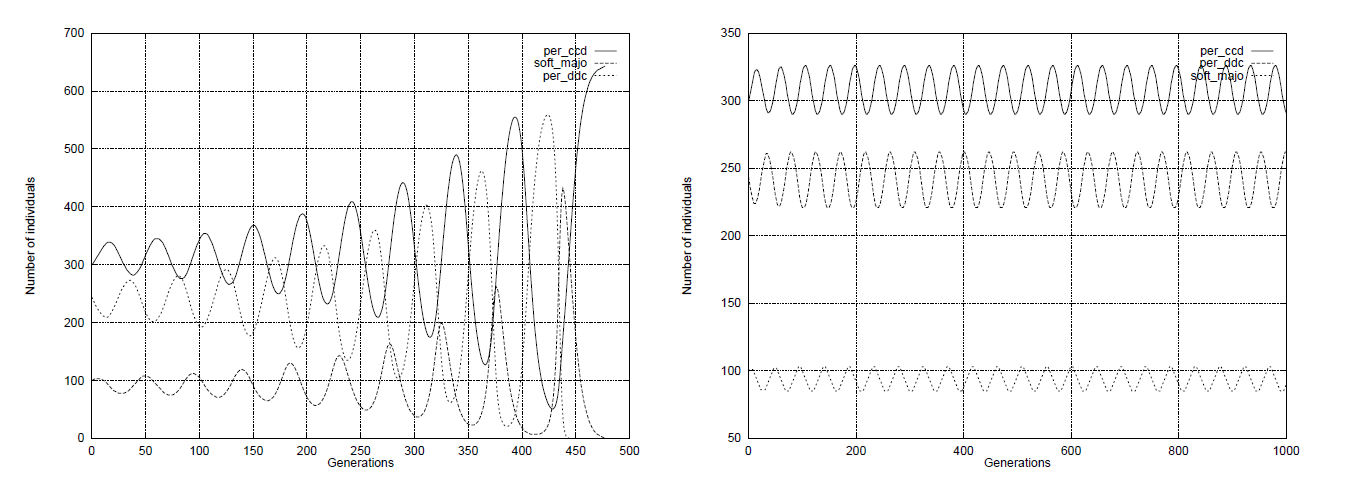
\includegraphics[width=1\linewidth]{sens_cipd}
	\end{minipage}
	\caption{Sensitivity to CIPD payoff. All parameters are identical except that \(T=4.6\)
		on the left and \( T=4.7\) on the right. (\texttt{sens\_cipd\_payoff.m})}
\end{figure}

\begin{figure}[ht!]
	\centering
	\begin{minipage}{1\textwidth}
		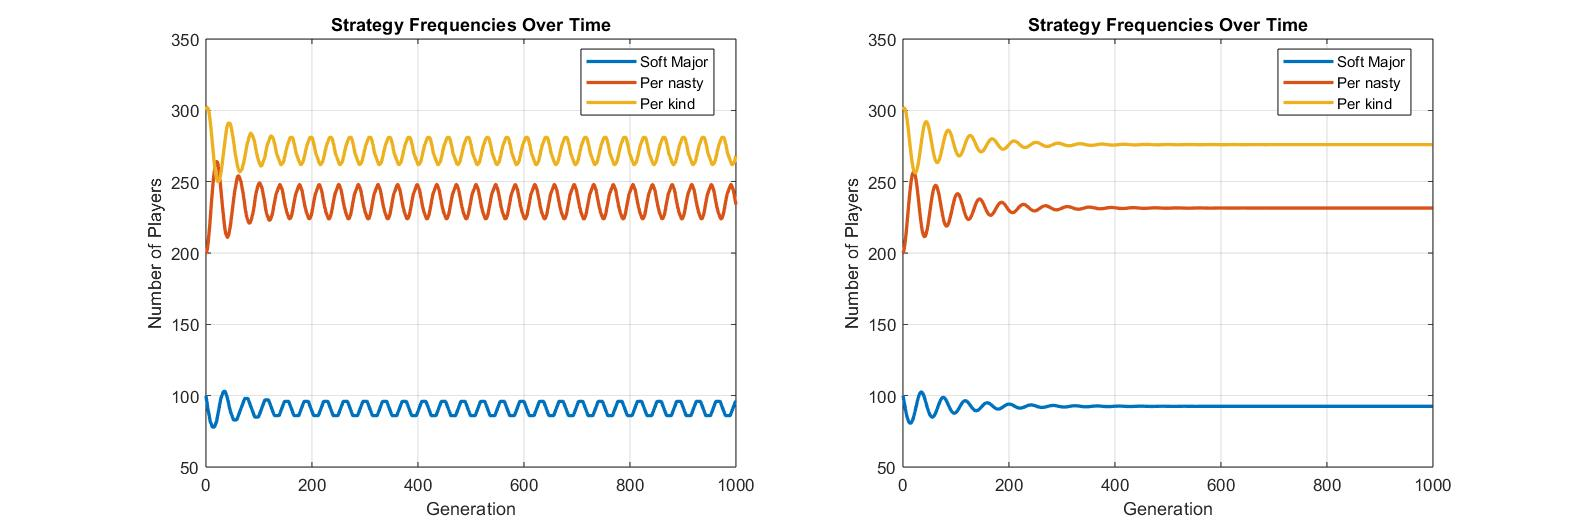
\includegraphics[width=1\linewidth]{fit_plots_theoretical/repartition_real}
		
		
	\end{minipage}
	\begin{minipage}{1\textwidth}
		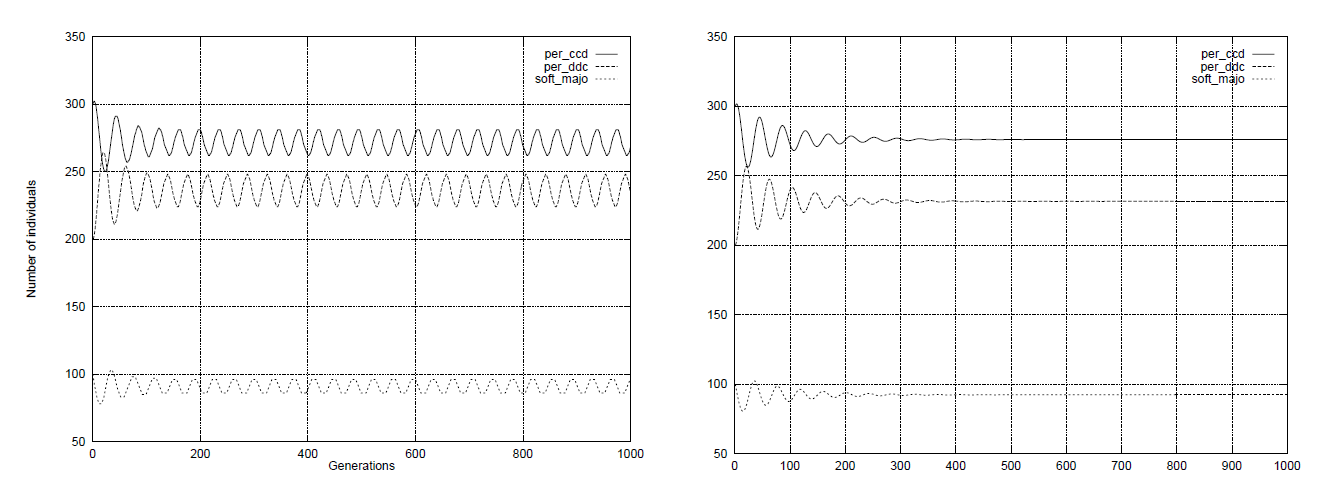
\includegraphics[width=1\linewidth]{sens_real}
	\end{minipage}
	\caption{Sensitivity to repartition computation method. All parameters are identical
		except that repartition on the left is done by rounding and uses real value on the right. (\texttt{sens\_repartition\_real.m})}
\end{figure}

\begin{figure}[ht!]
	\centering
	\begin{minipage}{1\textwidth}
		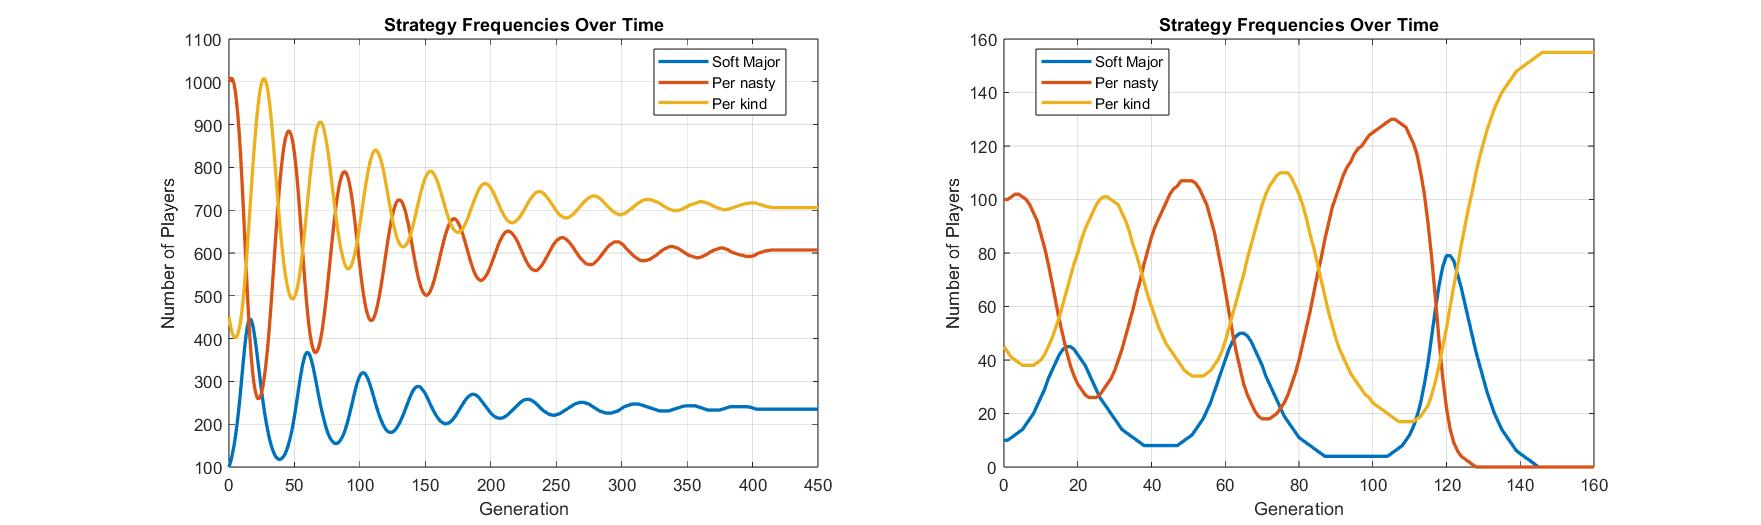
\includegraphics[width=1\linewidth]{fit_plots_theoretical/repartition_div10}
		
		
	\end{minipage}
	\begin{minipage}{1\textwidth}
		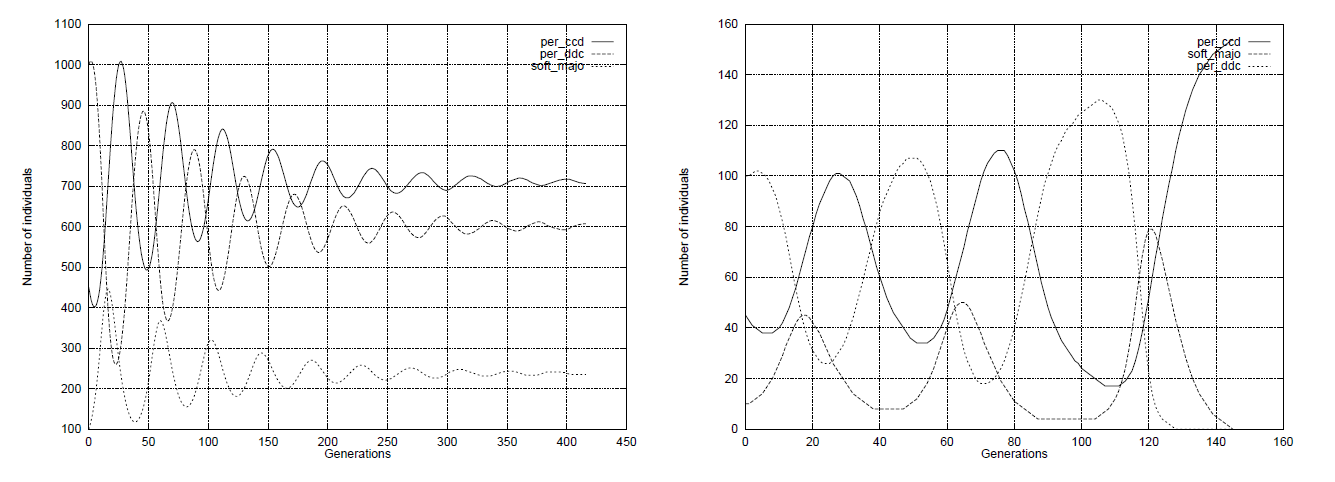
\includegraphics[width=1\linewidth]{sens_div10}
	\end{minipage}
	\caption{Sensitivity to repartition computation method. All parameters are identical
		except that populations on the right are divided by 10. (\texttt{sens\_repartition\_div10.m})}
\end{figure}


\clearpage

Παρατηρούμε την επ’ ακριβώς αντιστοίχιση με τα αποτελέσματα του paper ακόμα και σε επίπεδο debugging βλέποντας τους πίνακες των κερδών.
Στη συνέχεια επιχειρήσαμε να δημιουργήσουμε αυτές τις καμπύλες τρέχοντας προσομοιώσεις όπου είχαμε να αποφασίσουμε μεταξύ της πλήρους ή της μερικής προσομοίωσης.

\section{Προσομοίωση του Fitness Dynamics}
Στη συνέχεια επιχειρήσαμε να δημιουργήσουμε αυτές τις καμπύλες τρέχοντας προσομοιώσεις όπου είχαμε να αποφασίσουμε μεταξύ της πλήρους ή της μερικής προσομοίωσης.
Για τους σκοπούς αυτούς χρησιμοποιούμε τη συνάρτηση \nameref{appendix:TSF} η οποία αναλύεται παρακάτω:
\subsection{Θεωρητική Αναλυση του TourSimFit:
}




Η συνάρτηση αυτή είναι παρόμοια με την \texttt{TourTheFit} . Η βασική διαφορά είναι ότι για να διατηρηθεί ο πληθυσμός με ακέραιες τιμές χρησιμοποιούμε την συνάρτηση \nameref{appendix:CIV}


Η συνάρτηση αυτή ουσιαστικά μεταφέρει το περισσευούμενο fractional part στα στοιχεία με το χαμηλότερο fractional part. 
\\
\\
Σημαντική διαφορά εδώ είναι ότι , για να έχουμε μεγαλύτερη ταχύτητα στο Simulation, εκτελούμε τον κώδικα χρησιμοποιώντας την συνάρτηση \nameref{appendix:A2I}.
\\

Έτσι εκτελούμε μια μορφή half simulation (όχι καθαρή προσομοίωση). 
\\

Τρέχοντας ξανά τις παρακάτω προσομοιώσεις παρατηρούμε τα εξής για το κάθε ένα πείραμα.
\subsubsection{Defectors may be strong}

% TODO: \usepackage{graphicx} required
\begin{figure}[ht!]
\centering
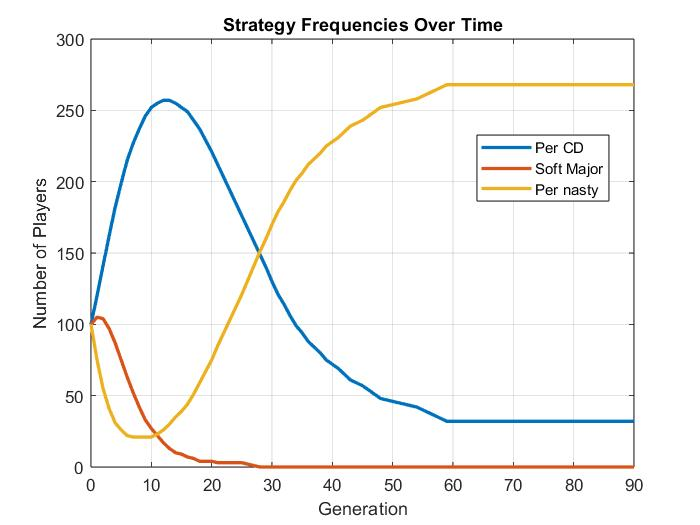
\includegraphics[width=0.5\linewidth]{fit_plots_simulations/defectors_may_be_strong_sim}
\caption{\texttt{defectors\_may\_be\_strong\_sim.m}}
\label{fig:defectorsmaybestrongsim}
\end{figure}

Παρατηρούμε παρόμοια συμπεριφορά με ίδιες γραφικές παραστάσεις με τη μόνη διαφορά η προσομοίωση να οδηγείται σε steady state μερικές γενιές νωρίτερα
\clearpage

\subsubsection{Monotonous Convergence}
% TODO: \usepackage{graphicx} required
\begin{figure}[th!]
\centering
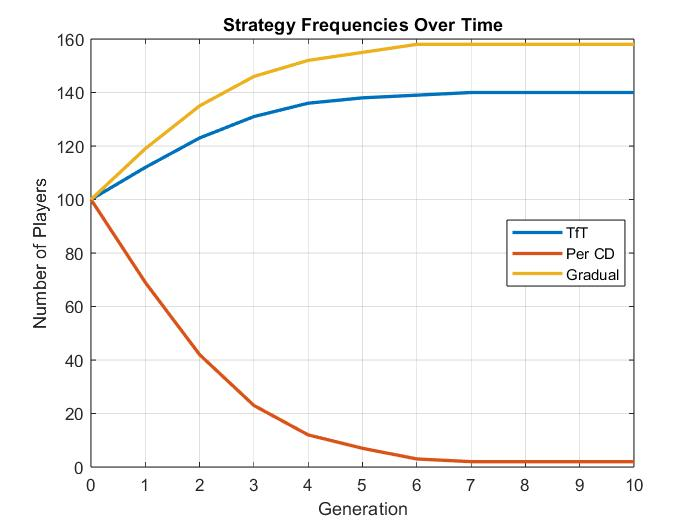
\includegraphics[width=0.7\linewidth]{fit_plots_simulations/monotonous_convergence_sim}
\caption{\texttt{monotonous\_convergence\_sim.m}}
\label{fig:monotonousconvergencesim}
\end{figure}

Παρατηρούμε και εδώ παρόμοια συμπεριφορά με ίδιες γραφικές παραστάσεις και ελαφρά αλλαγμένους τους πληθυσμούς του steady state.


\subsubsection{Attenuated Oscillations}
% TODO: \usepackage{graphicx} required
\begin{figure}[th!]
\centering
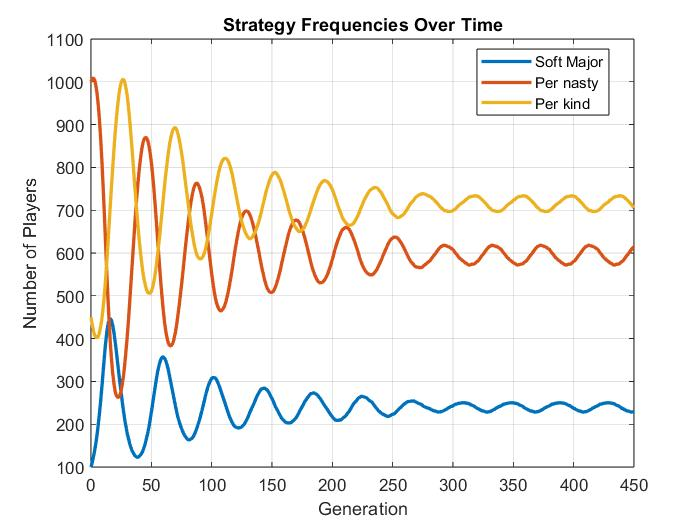
\includegraphics[width=0.7\linewidth]{fit_plots_simulations/attenuated_oscillatory_movements_sim}
\caption{\texttt{attenuated\_oscillatory\_movements\_sim.m}}
\label{fig:attenuatedoscillatorymovementssim}
\end{figure}

Παρατηρούμε παρόμοια συμπεριφορά με ίδιες γραφικές παραστάσεις με το simulation να έχει μικρότερο βαθμό απόσβεσης.


\subsubsection{Periodic Movements}
% TODO: \usepackage{graphicx} required
\begin{figure}[th!]
\centering
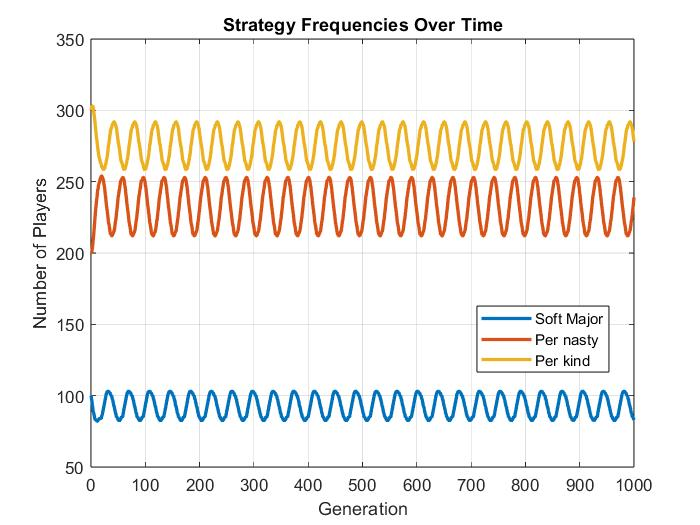
\includegraphics[width=0.7\linewidth]{fit_plots_simulations/periodic_movements_sim}
\caption{\texttt{periodic\_movements\_sim.m}}
\label{fig:periodicmovementssim}
\end{figure}

Παρατηρούμε παρόμοια συμπεριφορά με τη θεωρητική ανάλυση
\subsubsection{Increasing Oscillations}
% TODO: \usepackage{graphicx} required
\begin{figure}[th!]
\centering
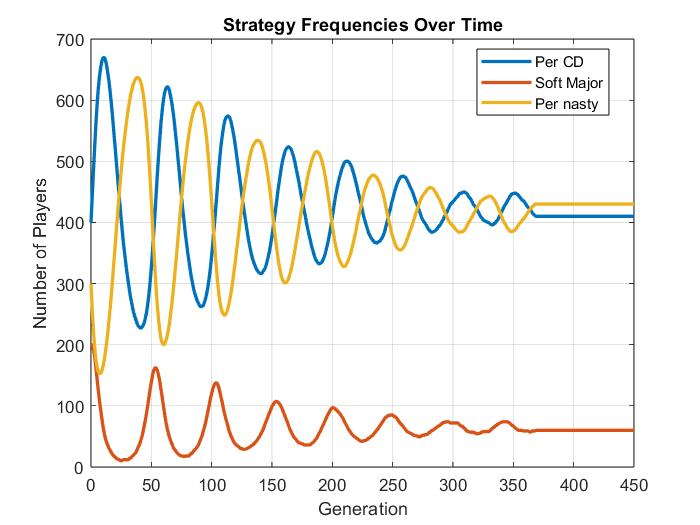
\includegraphics[width=0.7\linewidth]{fit_plots_simulations/increasing_oscillations_sim}
\caption{\texttt{increasing\_oscillations\_sim.m}}
\label{fig:increasingoscillationssim}
\end{figure}

Παρατηρούμε σημαντική διαφορά καθώς στην περίπτωση της προσομοίωσης δε συμβαίνουν αυξανόμενες ταλαντώσεις. Αυτό οφείλεται στον τρόπο που γίνεται το rounding στην προσομοίωση και εμφανίζεται και σε επόμενα πειράματα πολλές φορές χαλώντας και την κατάταξη των στρατηγικών. Στο συγκεκριμένο αν και οι ταλαντώσεις είναι μειούμενες η κατάταξη διατηρείται.
\subsubsection{Disordered Oscillations}
% TODO: \usepackage{graphicx} required
\begin{figure}[th!]
\centering
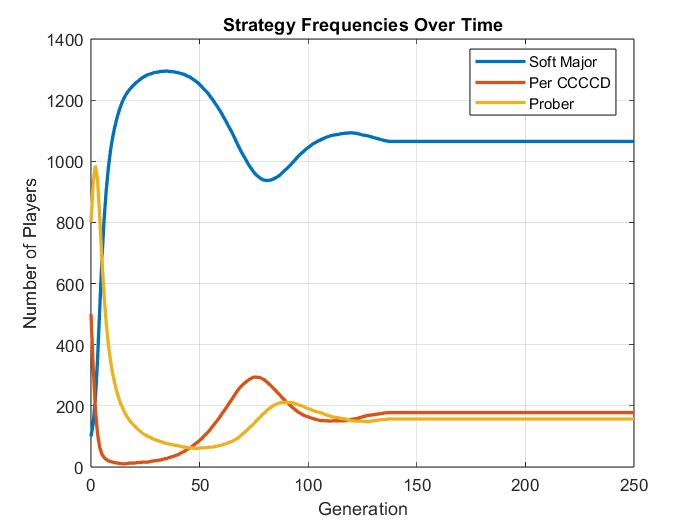
\includegraphics[width=0.7\linewidth]{fit_plots_simulations/disordered_oscillations_sim}
\caption{\texttt{disordered\_oscillations\_sim.m}}
\label{fig:disorderedoscillationssim}
\end{figure}

Παρατηρούμε παρόμοια συμπεριφορά με τη θεωρητική ανάλυση, ωστόσο οι μεταβολές είναι μικρότερες και καταλήγει σε λιγότερες γενιές σε steady state.
\subsubsection{Sensitivity of dynamics to population size}
% TODO: \usepackage{graphicx} required
\begin{figure}[ht!]
\centering
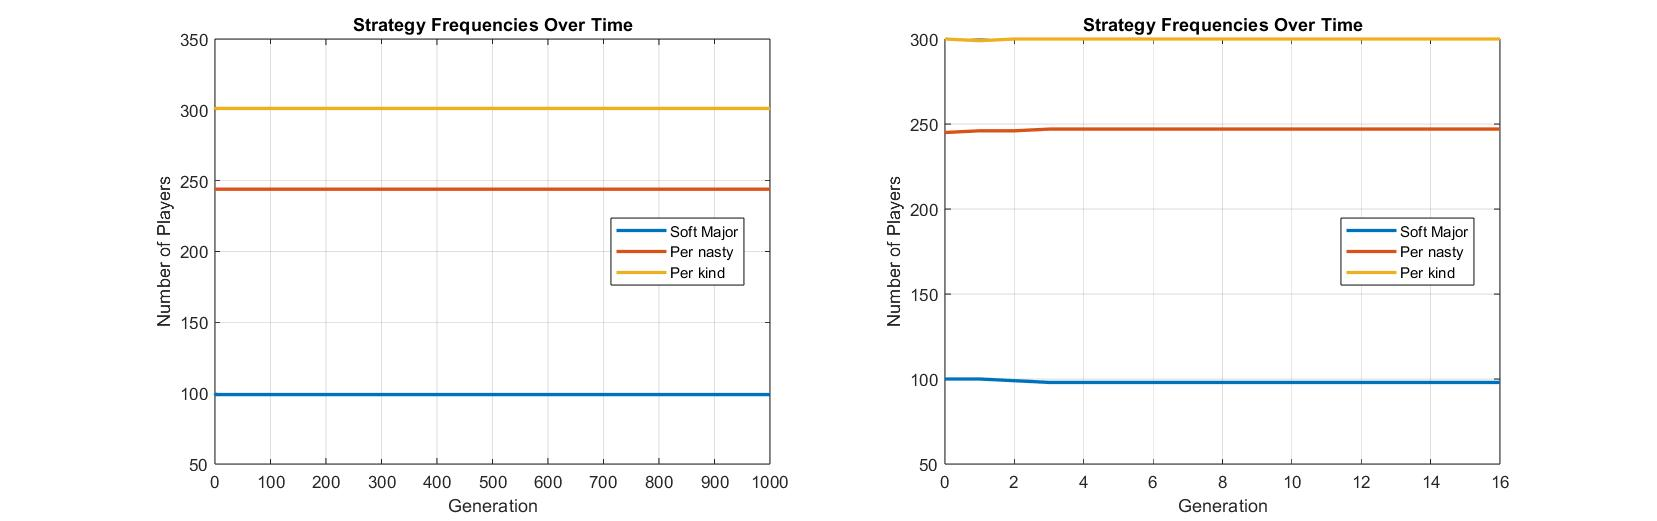
\includegraphics[width=1\linewidth]{fit_plots_simulations/sensitivity_to_population_size_sim}
\caption{\texttt{sens\_dyn\_pop\_size\_sim.m}}
\label{fig:sensitivitytopopulationsizesim}
\end{figure}

Παρατηρούμε ότι οι αρχικές συνθήκες που στην θεωρητική ανάλυση προκαλούν περιοδικές ταλαντώσεις στην προσομοίωση αποτελούν ήδη steady state.\clearpage
\subsubsection{Sensitivity of dynamics to winner}
% TODO: \usepackage{graphicx} required
\begin{figure}[th!]
\centering
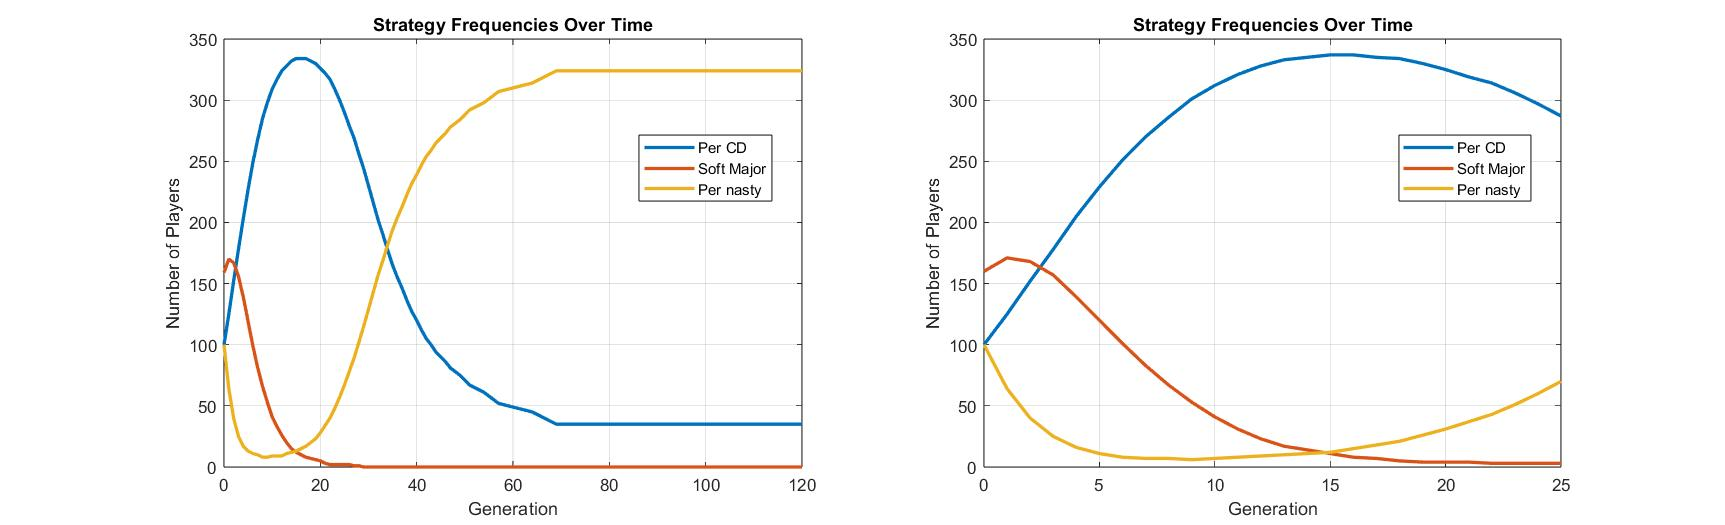
\includegraphics[width=1\linewidth]{fit_plots_simulations/sensitivity_of_winner_to_popsize_sim}
\caption{\texttt{sens\_win\_pop\_size\_sim.m}}
\label{fig:sensitivityofwinnertopopsizesim}
\end{figure}

Παρατηρούμε παρόμοια συμπεριφορά με τη θεωρητική ανάλυση

\subsubsection{Sensitivity to CIPD Payoff}




% TODO: \usepackage{graphicx} required
\begin{figure}[th!]
\centering
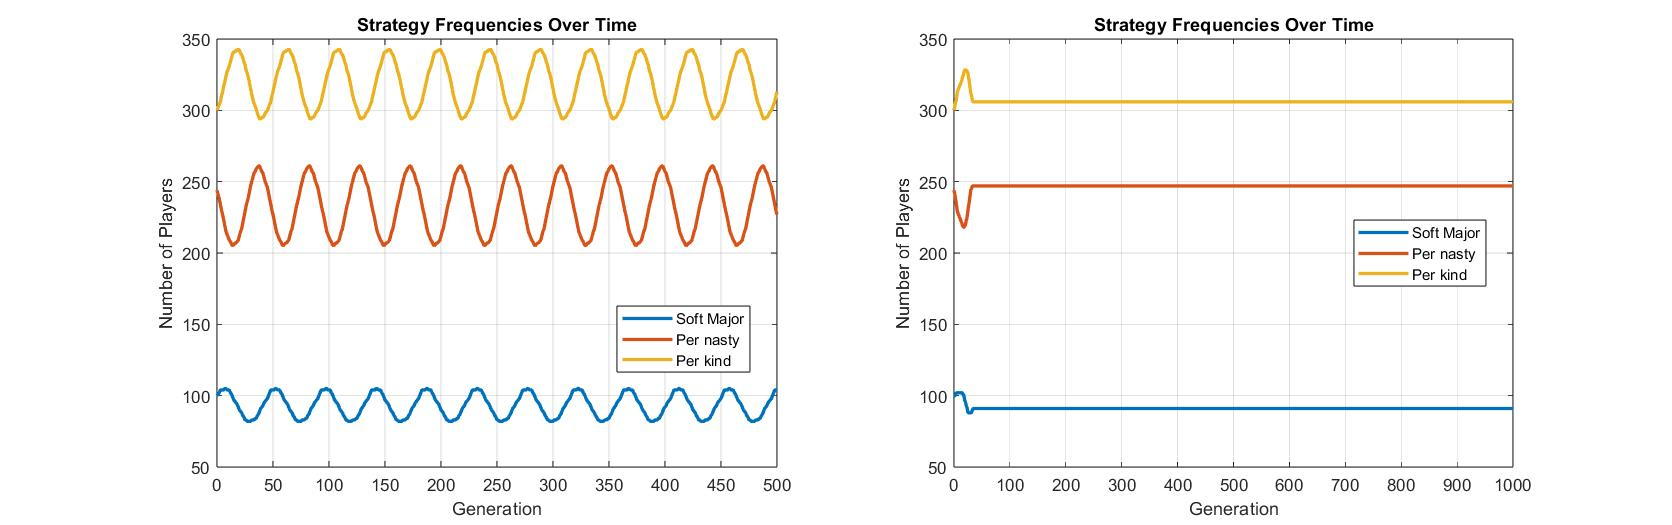
\includegraphics[width=1\linewidth]{fit_plots_simulations/sensitivity_to_cipd_payoff_sim}
\caption{\texttt{sens\_cipd\_payoff\_sim.m}}
\label{fig:sensitivitytocipdpayoffsim}
\end{figure}
Παρατηρούμε στη θεωρητική ανάλυση ότι με τις τιμές αυτές του πίνακα των σκορ έχουμε αυξανόμενες ταλαντώσεις και περιοδικές ταλαντώσεις ενώ στην προσομοίωση αντίστοιχα περιοδικές ταλαντώσεις και ένα σύντομο μεταβατικό φαινόμενο που οδηγεί σε steady state. 
\subsubsection{Sensitivity to Game Length}
% TODO: \usepackage{graphicx} required
\begin{figure}[th!]
\centering
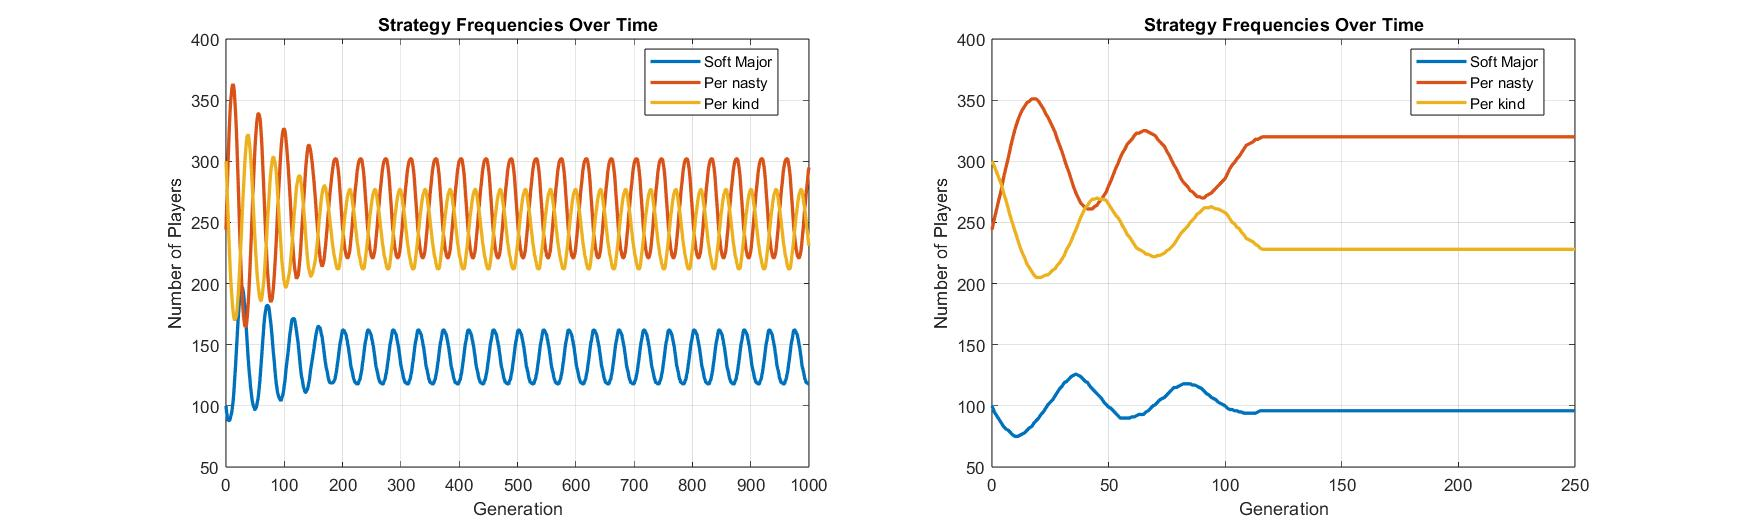
\includegraphics[width=1\linewidth]{fit_plots_simulations/sensitivity_to_game_length_sim}
\caption{\texttt{sens\_game\_length\_sim.m}}
\label{fig:sensitivitytogamelengthsim}
\end{figure}

Παρατηρούμε παρόμοια συμπεριφορά με τη θεωρητική ανάλυση

\subsubsection{Repartition divided by 10}
% TODO: \usepackage{graphicx} required
\begin{figure}[th!]
\centering
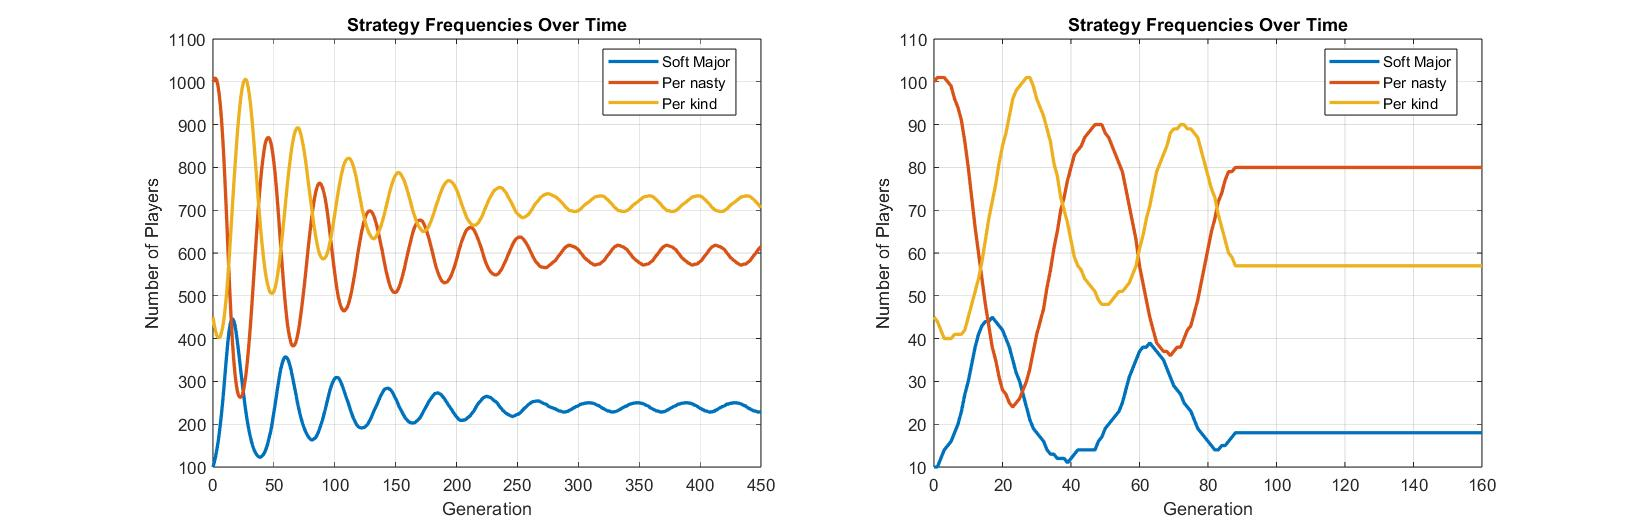
\includegraphics[width=0.7\linewidth]{fit_plots_simulations/repartition_div10_sim}
\caption{\texttt{sens\_repartition\_div10\_sim.m}}
\label{fig:repartitiondiv10sim}
\end{figure}

Παρατηρούμε πως ενώ στη θεωρητική ανάλυση είχαμε μειούμενες και αυξανόμενες ταλαντώσεις στην προσομοίωση έχουμε και στις δύο περιπτώσεις μειούμενες ταλαντώσεις οι οποίες όμως στην περίπτωση της διαίρεσης  με το 10 των πληθυσμών ανατρέπουν και την κατάταξη των στρατηγικών.





\chapter{Imitation Dynamics}
	\section{Θεωρητική ανάλυση του Imitation Dynamics:}
	
	Σε αυτό το σημείο θα αναλύσουμε τη θεωρητική ανάλυση του Imitation Dynamics.  Aυτό περιλαμβάνει την δημιουργία ενός πίνακα μεταβάσεων μιας αλυσίδας Markov. Παρακάτω θα αναλύσουμε πως λειτουργεί αυτή η μέθοδος παραγωγής του πίνακα μεταβάσεων.
	\\
	
	Παρακάτω ο κώδικας της συνάρτησης \nameref{appendix:TTI}:
	\\

	
	
	\indent Παμε να δουμε αναλυτικά γραμμή προς γραμμή:
	
	Αρχικα καλούμε την συνάρτηση \nameref{appendix:ACS}, η οποία δίνει όλες τις πιθανές καταστάσεις της διαδικασίας Markov, της οποίας τον πίνακα μεταβάσεων αναζητούμε .
	\\
	
	

	


	\vspace{1em}
	
	Η συνάρτηση ακολουθεί την λογική του \textit{stars and bars problem} για να υπολογίσει ολους τους πιθανούς συνδυασμούς θετικών αριθμων που αθροίζουν στον πληθυσμο που έχουμε βάλει σαν όρισμα.
	\\
	\\
	Προχωρώντας στις επόμενες γραμμές: Αρχικοποιούμε τον πίνακα μεταβάσεων και ξεκινάμε μια \texttt{for} loop για κάθε γραμμή του πίνακα, (δηλαδή για κάθε συνδυασμό των combos).
	\\
	\\
Εντός της λούπας: Υπολογίζουμε τα scores για κάθε στρατηγική με την συνάρτηση \nameref{appendix:A2I}.
\\
\\
	Η βελτιωμένη αυτή εκδοση αξιοποιεί την ανάλυση από το \texttt{TourTheFit} για να υπολογίσει με μεγαλύτερη ταχύτητα τα Scores για κάθε στρατηγική.

	Επειτα , με την συνάρτηση \nameref{appendix:FBIS} βρίσκω τις στρατηγικές (μια η περισσότερες) που είναι βέλτιστες. Επιπλέον υπολογίζει και τις υποβελτιστες στρατηγικές(θα μας χρησιμεύσουν μετα).\\
	

	Προχωρώντας, χρησιμοποιώντας την \nameref{appendix:ASstr} , την οποία έχουμε υλοποιήσει για το πρωτάθλημα Axelrod της 1ης εργασίας, μετατρέπουμε την μορφή:
	
	\[X(t_i)=\Bigl(x_1(t_i),x_2(t_i),\dotsc,x_m(t_i)\Bigr)\to Y(t_i)=\underbrace{\texttt{str}_1,\dots\texttt{str}_1}_{x_1(t_i) \text{ times }}\ , \ \underbrace{\texttt{str}_2,\dots\texttt{str}_2}_{x_2(t_i) \text{ times }}\ , \dots,\underbrace{\texttt{str}_m,\dots\texttt{str}_m}_{x_m(t_i) \text{ times }} \]
	\\
	Η μορφή αυτή εξυπηρετεί τους εξής σκοπούς:
	\begin{itemize}
		\item Είναι ευκολότερη η εύρεση πιθανών μεταβολών παιχτών
		\\
		\item Δεν μας ενδιαφέρει η διάταξη των στοιχείων. Όπως είχαμε αναφέρει στο μάθημα, η διαδικασία markov για τις καταστάσεις \(Y\) (ας τις ονομάσουμε \texttt{r\_states} έναντι των \texttt{s\_states}) είναι lumpable σε σχέση με τα
		\texttt{s\_states} \footnote{βλέπε στο Appendix για λεπτομέρειες} Αυτό σημαίνει ότι το άθροισμα των πιθανοτήτων μεταβολών ενος συγκεκριμένου \texttt{group r\_states} που αναπαριστούν ένα συγκεκριμένο \texttt{s\_state} είναι σταθερό από  οποιαδήποτε άλλη κατάσταση ενος συγκεκριμένου \texttt{s\_state} και να προερχόμαστε.
		
		
	\end{itemize}

	Παρακάτω, εφόσον έχουμε τώρα το \texttt{r\_state}, υπολογίζουμε τα \textit{indexes} που αντιστοιχούν σε βέλτιστες και υποβέλτιστες στρατηγικές. Εδώ κάνουμε και μια παραδοχή για να μπορέσει ο μηχανισμός μας να αντιμετωπίσει ειδικες περιπτώσεις: Εφόσον ο αριθμός υποβέλτιστων παιχτών είναι μικρότερος από \(Κ\), τότε σαν υποψήφιοι παίκτες προς αλλαγή στρατηγικής συμπεριλαμβάνονται και οι βελτιστοι παίκτες(δηλαδή όλοι οι παίκτες είναι υποψήφιοι για αλλαγή στρατηγικής, ανεξαρτήτως αν έχουν ήδη βέλτιστη στρατηγική).
\\
	
	
	Εφόσον έχουμε βρει τα indexes , αναπαράγουμε ολους τους πιθανούς συνδυασμούς indexes από το \texttt{idx\_r} μήκους \(K\) και όλους τους πιθανούς συνδυασμούς βέλτιστων στρατηγικών που μπορούν να μεταβληθούν οι \(Κ\) παίκτες. Για το 2ο έχουμε υλοποιήσει μια συνάρτηση για να βρεί όλους τους πιθανούς συνδυασμούς με επανατοποθέτηση.
	

	
Η συνάρτηση αυτή μάλλον χρήζει βελτίωσης, αφού στην συγκεκριμένη μορφή της είναι αναδρομική.
	\\
\\
	Σε αυτό το σημείο ξεκινάνε οι υπολογισμοί στοιχείων του πίνακα μεταβάσεων. Ορίζουμε με την βοήθεια ενός cell array όλες τις πιθανές μεταβάσεις (σε μορφή \texttt{r\_state}) από την παρούσα κατάσταση. Επειτα βρίσκω σε ποιό \texttt{s\_state} αντιστοιχεί το κάθε \texttt{r\_state} και στο αντίστοιχο στοιχείο \(s\to s'\) προσθέτω \(\frac{1}{p}\), όπου \(p\) o πιθανός αριθμός των μεταβάσεων \texttt{r\_states}.	
\\
\\

Θα δοκιμάσουμε μερικά παραδείγματα με την συνάρτηση αυτή. ( \nameref{appendix:TTI} )
\\ 



Η συνάρτηση έχει αρκετά γρήγορη ταχύτητα ακόμα και για μεγάλο πληθυσμό ή μήκος στρατηγικών. Θα δοκιμάσουμε ενα παράδειγμα με 5 παίκτες \texttt{Per\_CD} , 5 παίκτες \texttt{Soft\_Major} και 5 παίκτες \texttt{Per\_Nasty}.
% TODO: \usepackage{graphicx} required
\begin{figure}[th!]
	\centering
	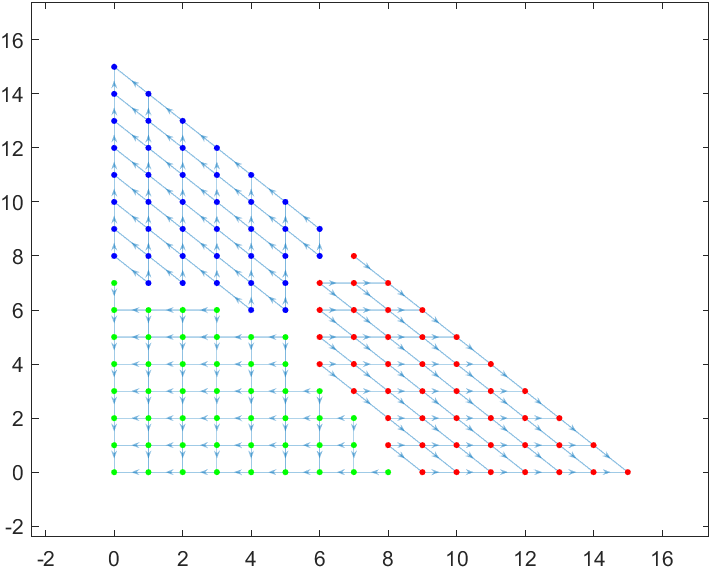
\includegraphics[width=0.7\linewidth]{TourTheImi_Ex1}
	\caption{\texttt{TourTheImi} Ex. 1\\ \texttt{ TourTheImi\_Ex1.m}}
	\label{fig:tourtheimiex1}
\end{figure}

	% TODO: \usepackage{graphicx} required

Βλέπουμε ότι ο γράφος χωρίζεται σε ξεχωριστά groups ανάλογα με την σύγκλιση τους . Φαίνεται πως υπάρχει μια 1 προς 1 σχέση μεταξύ της αρχικής και τελικής κατάστασης(μπορούμε να γνωρίζουμε σίγουρα που θα καταλήξει μια κατάσταση από την αρχική κατάσταση και μόνο)
\\
Έπειτα κάνουμε ένα πείραμα με 5 \texttt{TfT}, 5 \texttt{Per\_CD}, 5 \texttt{Gradual}
% TODO: \usepackage{graphicx} required
\begin{figure}[th!]
	\centering
	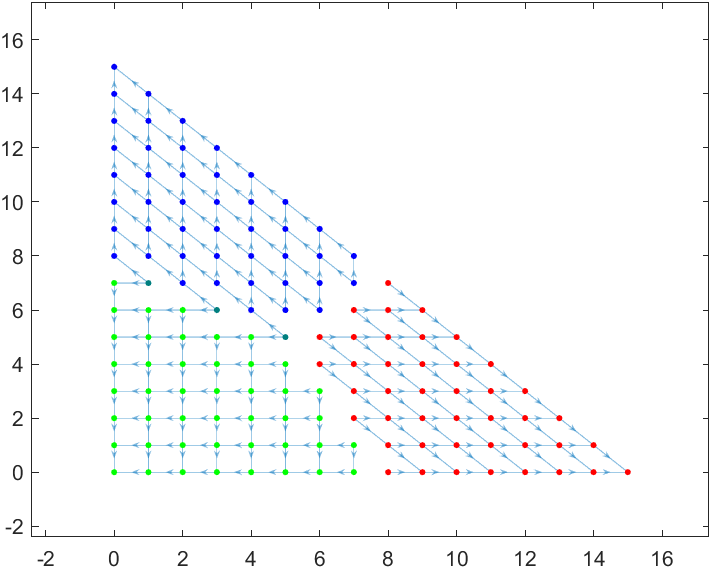
\includegraphics[width=0.7\linewidth]{TourTheImi_Ex2}
	\caption{\texttt{TourTheImi } Ex. 2    \texttt{TourTheImi\_Ex2.m}}
	\label{fig:tourtheimiex2}
\end{figure}

Εδώ βλέπουμε ότι, παρόλο που ο γράφος πάλι χωρίζεται σε groups, υπάρχει μια επικοινωνία μεταξύ των 2 από τα 3 groups . Συγκεκριμένα , οι καταστάσεις \([7,1,7]\) ,\([6,3,6]\) και \([5,5,5]\) έχουν πιθανότητα να οδηγηθεί τόσο στην κατάσταση \([15,0,0]\) όσο και στην κατάσταση \([0,0,15]\). Αυτό λογικά συμβαίνει καθώς οι στρατηγικές \texttt{Tit\_for\_Tat} και \texttt{Gradual} έχουν ίδιο συνολικό score και στις 3 αυτές καταστάσεις.\\
\\

Το επόμενο πείραμα αποτελείται από 3 \texttt{Soft\_major}, 2 \texttt{Per\_Nasty}, 1 \texttt{Per\_kind}.
% TODO: \usepackage{graphicx} required
\begin{figure}[th!]
	\centering
	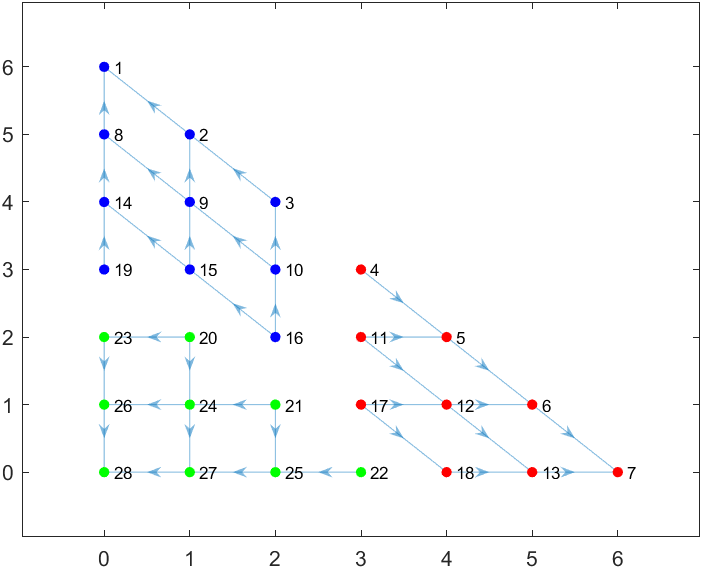
\includegraphics[width=0.6\linewidth]{TourTheImi_Ex3}
	\caption{\texttt{TourTheImi } Ex. 3 \texttt{ TourTheImi\_Ex3.m }}
	\label{fig:tourtheimiex3}
\end{figure}



Για την συνάρτηση \texttt{TourTheimi} δημιουργήσαμε μια δεύτερη παραλλαγή \nameref{appendix:TTI2} με τον εξής συλλογισμό: Το Score ενος πληθυσμού δεν θα έπρεπε να κρίνεται από τον αριθμό που τον εκπροσωπεί αλλά από την απόδοση ενός παίκτη.



Η μεγάλη διαφορά της \texttt{TourTheimi2} είναι ότι χρησιμοποιεί μια νέα συνάρτηση ( \nameref{appendix:Axel2Imp2}) για τον υπολογισμό του Score ανα στρατηγική , η οποία λαμβάνει υπόψη το Score μόνο ενός παίκτη.
\\
\\
Παμε να εξετάσουμε τα ίδια παραδείγματα με πάνω με την νέα συνάρτηση.
\\
\\
Δοκιμάζουμε με 5 \texttt{per\_CD},5 \texttt{soft\_major}, 5 \texttt{per\_nasty}.\\
\\
% TODO: \usepackage{graphicx} required
\begin{figure}[th!]
	\centering
	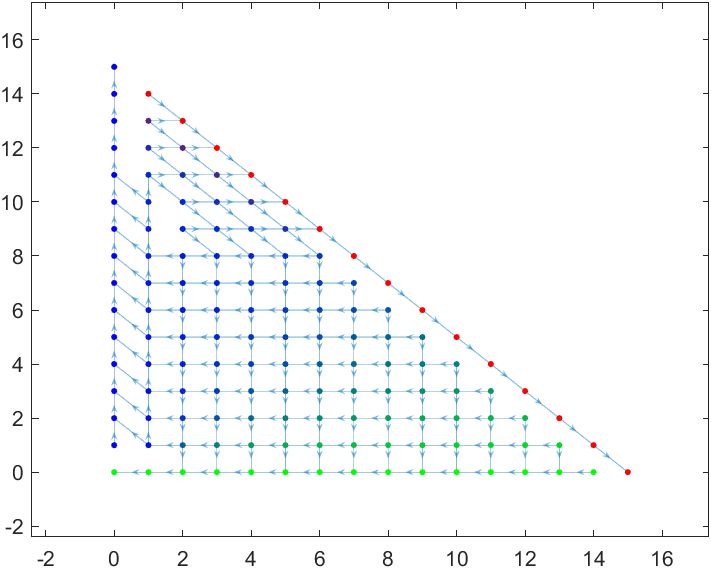
\includegraphics[width=0.7\linewidth]{TourTheImi_Ex1_2}
	\caption{\texttt{TourTheImi} Ex1\_2 \texttt{TourTheImi\_Ex1\_2.m}}
	\label{fig:tourtheimiex12}
\end{figure}
\\
Παρατηρούμε οτι το \texttt{TourTheImi2} έχει μεγάλη διαφοροποίηση. Εδω βλέπουμε ότι ο γράφος δεν χωρίζεται τόσο αισθητά σε Groups. Αυτό μας δείχνει πως υπάρχουν ισοδύναμες στρατηγικές στο συγκεκριμένο παράδειγμα.
\clearpage

Έπειτα έχουμε 5 \texttt{TfT}, 5 \texttt{Per\_CD}, 5 \texttt{Gradual}.
% TODO: \usepackage{graphicx} required
\begin{figure}[th!]
	\centering
	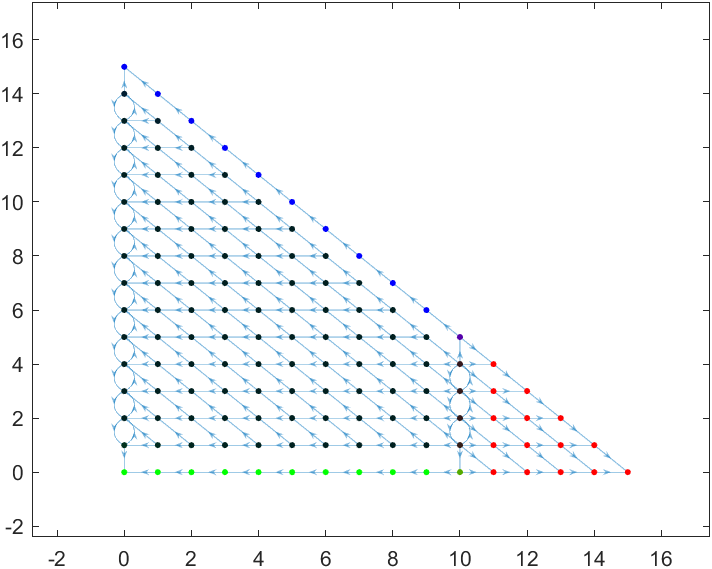
\includegraphics[width=0.7\linewidth]{TourTheImi_Ex2_2}
	\caption{\texttt{TourTheImi} Ex2\_2    \texttt{ TourTheImi\_Ex2\_2.m}}
	\label{fig:tourtheimiex22}
\end{figure}

Στο συγκεκριμένο παράδειγμα παρατηρούμε ότι στην περίπτωση που η στρατηγική \texttt{ Per\_CD} εκλείψει, οι στρατηγικές \texttt{Tit\_for\_Tat} και \texttt{Gradual} ταλαντεύονται στο ποιά θα υπερισχύσει. Επιπλέον στις καταστάσεις \([1,10,4]\),\([2,10,3]\),\([3,10,2]\) και \([4,10,1]\) βλέπουμε ότι από αυτές τις καταστάσεις μπορούμε να μετακινηθούμε προς πολλές κατευθύνσεις.\\
\\
Επόμενο πείραμα: 3 \texttt{Soft\_Major}, 2 \texttt{Per\_Nasty}, 1 \texttt{Per\_kind}

\begin{figure}[th!]
	\centering
	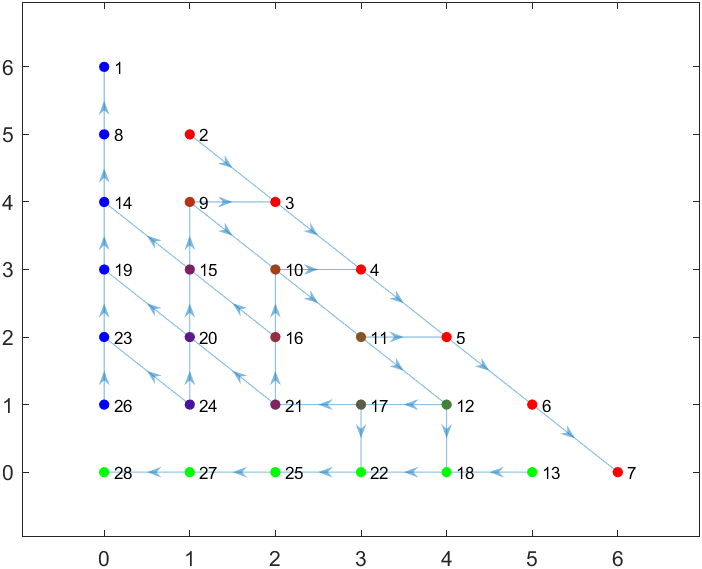
\includegraphics[width=0.60\linewidth]{TourTheImi_Ex3_2}
	\caption{\texttt{TourTheImi} Ex3\_2 \texttt{TourTheImi\_Ex3\_2.m}}
	\label{fig:tourtheimiex32}
	\flushleft
	Οπως και πριν , δεν παρατηρούμε κάτι ιδιαίτερο στο συγκεκριμένο πείραμα , ακόμα και με το TourTheImi2.
\end{figure}







\section{Προσομοίωση του Imitation Dynamics}
Ο κώδικας για το Simulation του Imitation Dynamics βρίσκεται εδω:\nameref{appendix:TourSimImi}
    
Η λογική είναι παρόμοια με την \nameref{appendix:TTI}, με την διαφορά ότι αυτή τη φορά δεν χρειάζεται να υπολογίσουμε τον πίνακα μεταβάσεων: Επιλέγουμε τυχαία \(Κ\) παίκτες και επιλέγουμε τυχαία μια από τις βέλτιστες στρατηγικές για να αλλάξουμε τους \( Κ\) παίκτες.
\\
\\
Εκτελώντας τα αντίστοιχα πειράματα με τη θεωρητική υλοποίηση παρατηρούμε ότι στην περίπτωση του Imitation όπου η βέλτιστη στρατηγική βρίσκεται από το συνολικό σκορ όλών των παικτών η συμπεριφορά του συστήματος εμφανίζει τις παρακάτω ιδιομορφίες:

\begin{enumerate}
\item  Στην περίπτωση που ένας πληθυσμός είναι αρχικά μεγαλύτερος από έναν άλλο, ο πληθυσμος τείνει να υπερισχύει έναντι των άλλων, όπως βλέπουμε στην 3η εικόνα που εκτελείται το χαοτικό πείραμα.

\item  Στην περίπτωση που οι πληθυσμοί είναι ίδιοι, τείνει να υπερισχύει αυτός που σε σχέση με το Theoretical Fitness εμφανίζει την πιο πρώιμη αύξηση. Αυτό μπορεί να οδηγήσει τόσο σε ορθή κατάταξη , όπως στην 2η εικονα στο πείραμα της μονότονης σύγκλισης, όσο και σε λανθασμένη , όπως στην πρώτη εικόνα με το πείραμα των ισχυρών αποστατών.


\end{enumerate}
Στην περίπτωση του Imitation όπου η βέλτιστη στρατηγική βρίσκεται από το σκορ του καλύτερου παίκτη, τα αποτελέσματα παρουσιάζονται πιο χαοτικά και δεν υπάρχει απαραίτητα μονοτονία στις μεταβολές όπως παρατηρείται στην πρώτη περίπτωση.\\
\\
% TODO: \usepackage{graphicx} required
\begin{figure}[!th]
	\centering
	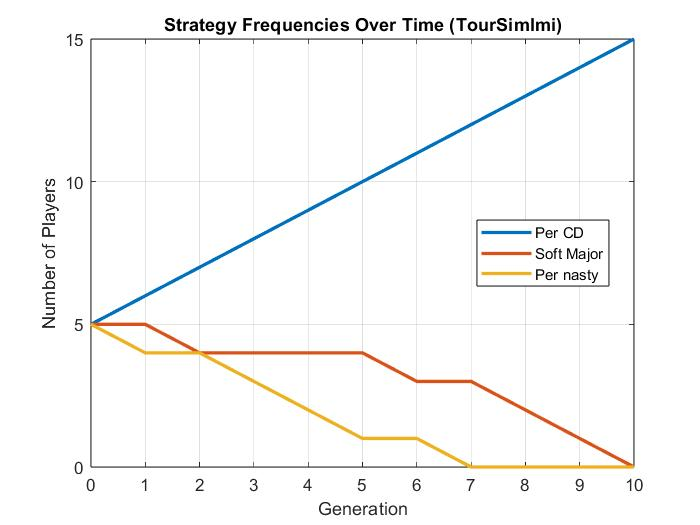
\includegraphics[width=0.7\linewidth]{toursimimi1}
	\caption{Convergence to the Final State \texttt{TourSimImi\_Ex1.m}}
	\label{fig:toursimimi1}
\end{figure}
% TODO: \usepackage{graphicx} required
\begin{figure}[ht!]
	\centering
	\begin{minipage}{0.48\textwidth}
		\centering
		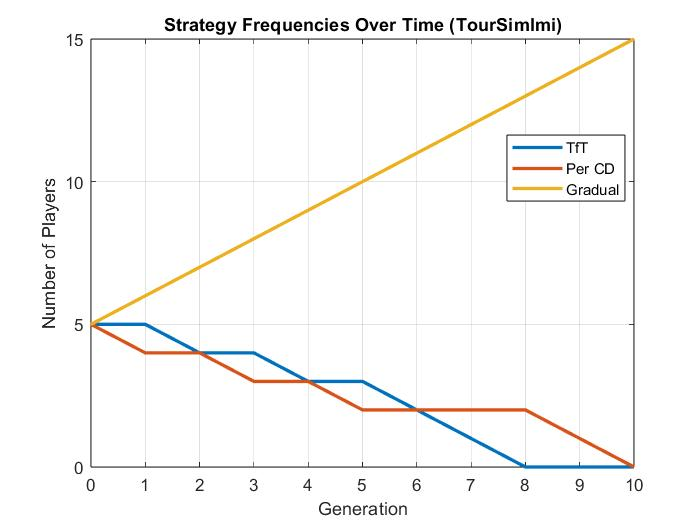
\includegraphics[width=0.8\linewidth]{toursimimi2}
	
	
	\end{minipage}
	\hfill
	\begin{minipage}{0.48\textwidth}
		\centering
		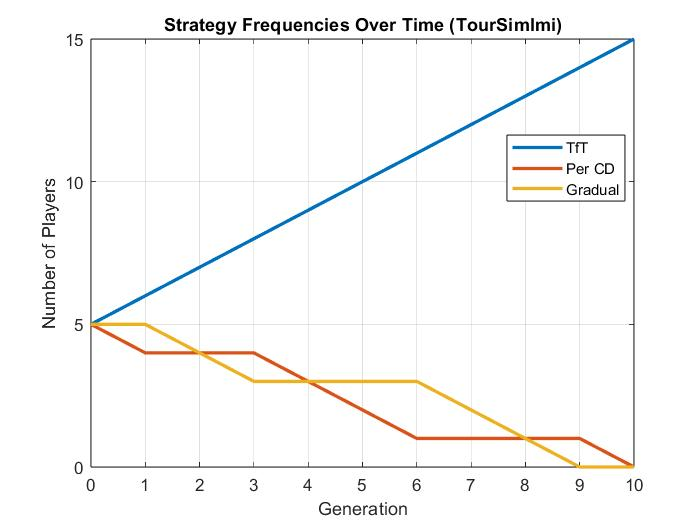
\includegraphics[width=0.8\linewidth]{toursimimi22}
	
	
	\end{minipage}
	\caption{Convergence of the states to the two possible final states shown by Markov Chain \texttt{  TourSimImi\_Ex2.m  }}
\end{figure}
% TODO: \usepackage{graphicx} required
\begin{figure}
	\centering
	
	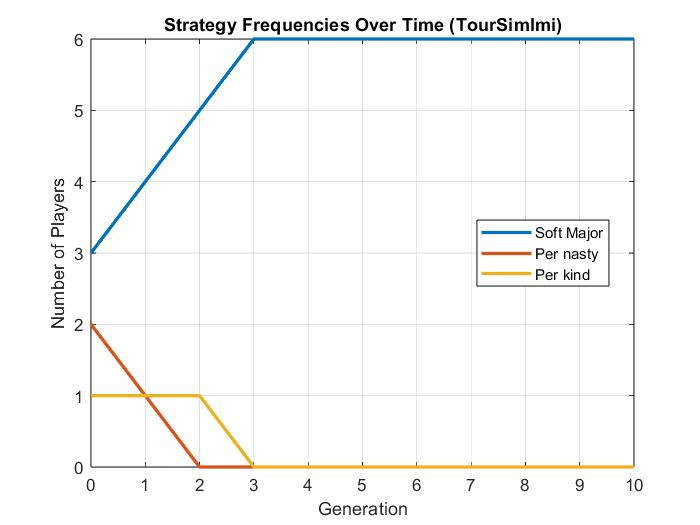
\includegraphics[width=0.7\linewidth]{toursimimi3}
	\caption{Convergence to the Final State   \texttt{(TourSimImi\_Ex3.m)}}
	\label{fig:toursimimi3}
\end{figure}
\clearpage
% TODO: \usepackage{graphicx} required
\begin{figure}
	\centering
	\begin{minipage}{0.48\textwidth}
		\centering
		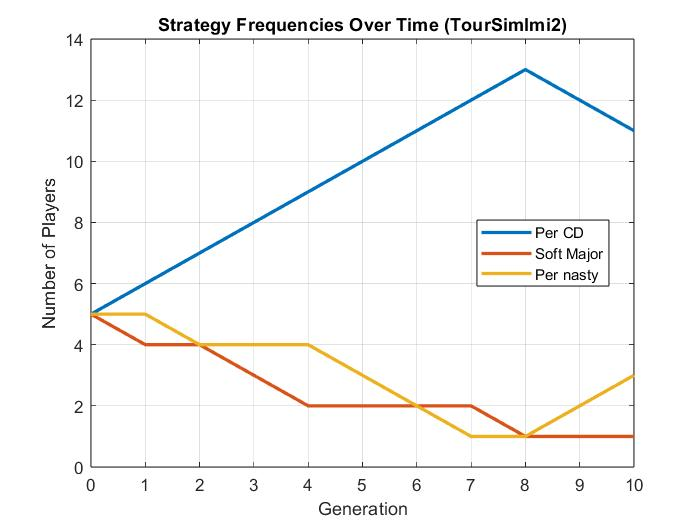
\includegraphics[width=0.7\linewidth]{toursimimi11.jpg}
	
		\label{fig:toursimimi11}
		
	\end{minipage}
		\begin{minipage}{0.48\textwidth}
			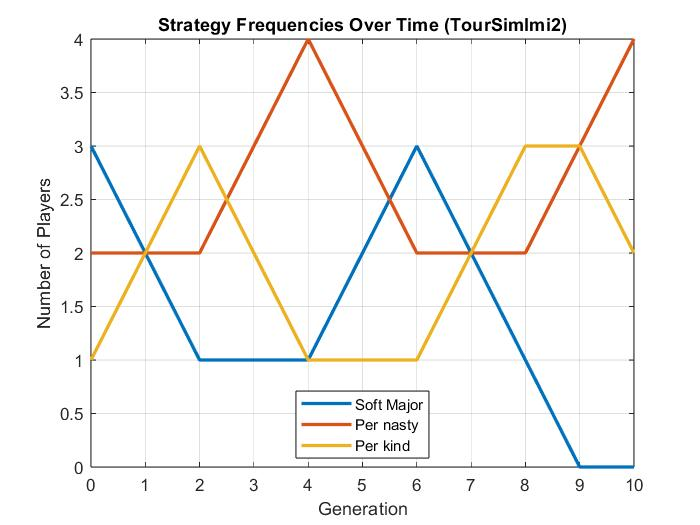
\includegraphics[width=0.7\linewidth]{toursimimi33}
			
		\end{minipage}
	
		\begin{minipage}{0.48\textwidth}
			\centering
		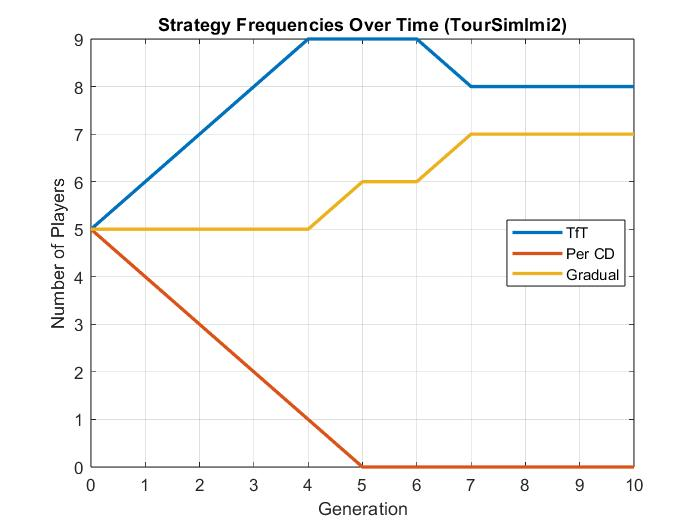
\includegraphics[width=0.7\linewidth]{toursimimi222}
	
	
	\end{minipage}
	\centering	
		\begin{minipage}{0.48\textwidth}
		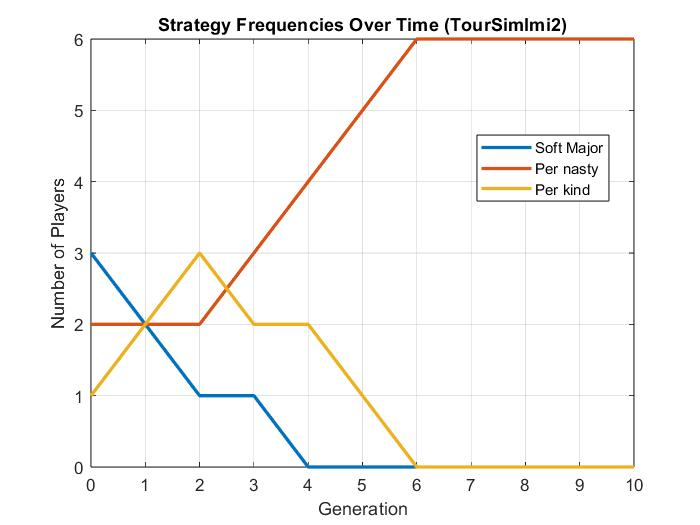
\includegraphics[width=0.7\linewidth]{toursimimi333}
		
	\end{minipage}
		\begin{minipage}{0.48\textwidth}
		\centering
		\includegraphics[width=0.7\linewidth]{toursimimi2222}
		
	\end{minipage}
	\caption{Increased Oscilations and random state transition using \texttt{TourSimImi2} \texttt{TourSimImi\_Ex1\_2.m, TourSimImi\_Ex2\_2.m,  TourSimImi\_Ex3\_2.m }}
\end{figure}

\chapter{Discussion}
Μέσα από την θεωρητική ανάλυση του Fitness Dynamics παρατηρούμε την ακριβή επαλήθευση των αποτελεσμάτων του paper καθώς και την επαλήθευσή τους σε πραγματικό χρόνο από την προσομοίωση. 
\\

Σε κάθε περίπτωση οι αρχικές συνθήκες παίζουν πολύ σημαντικό ρόλο και δόθηκε αρκετός χρόνος στην επίτευξη των ακριβών αποτελεσμάτων. Στη συνέχεια από το Imitation Dynamics παρατηρούμε την σύγκλιση των πληθυσμών προς σταθερές καταστάσεις μέσα από τις αλυσίδες Markov και πώς μερικές φορές από μια αρχική κατάσταση είμαστε βέβαιοι ότι στο τέλος θα οδηγηθούμε σε μια συγκεκριμένη τελική ενώ άλλες όχι. Τα βήματα προς την τελική κατάσταση από το Simulation των Imitation Dynamics εξαρτώνται και αυτά από διάφορους μηχανισμούς όπως την επιλογή βέλτιστης στρατηγικής και τον μηχανισμό επιλογής των παικτών προς αλλαγή. Σε αυτό το σημείο και καθώς δόθηκε αρκετή ελευθερία στην μοντελοποίηση του συστήματος τα αποτελέσματα μας ενδέχεται να διαφέρουν σε σχέση με τις υπόλοιπες ομάδες, ενώ καθώς ο τρόπος επιλογής παικτών προς αλλαγή περιλαμβάνει στοχαστικότητα τα figures που συμπεριλάβαμε ενδέχεται να μη παραχθούν ολόιδια με τα scripts ασχέτως αν ο μηχανισμός παραμένει κοινός.\\ 
Τέλος, η ανάλυση αυτή μπορεί να δώσει χρήσιμα συμπεράσματα τόσο για τα δυναμικά φαινόμενα στα εξελικτικά πρωταθλήματα ενώ σημαντικό ερευνητικό ενδιαφέρον θα παρουσίαζε η εφαρμογή της παραπάνω ανάλυσης και στα άλλα 2 διαφορετικά κοινωνικά διλλήματα τα οποία είναι οι Ιέρακες και Περιστερές και το Κυνήγι του Ελαφιού με αντίστοιχες προσαρμογές.
\begin{appendices}
\renewcommand{\thesection}{Appx. \Alph{section}:}

\section{\\Απόδειξη μεταξύ \texttt{s\_states }, \texttt{r\_states} από κ. Κεχαγιά  }
\subsection*{The General Case \( N \in \mathbb{N} \)}

As already mentioned, the process \((\bm{r}(t))_{t=0}^{\infty}\) is a MC. Let us now look at the \((s(t))_{t=0}^{\infty}\) process. We have  
\[
\forall t : \bm{s}(t) = F(\bm{r}(t)).
\]

We note that the inverse \(F^{-1}\) is a set-valued function:  
\[
\forall\bm{ s} : F^{-1}(\bm{s}) = \{ \bm{r} : F(\bm{r}) = \bm{s} \}.
\]

The following Definition 1 and Proposition 1  are from \cite{kex}.

\subsection*{Definition 1}
Suppose we are given: (a) a Markov chain \((\bm{x}(t))_{t=0}^{\infty}\) with state space \(R = \{ 1, \ldots, N \}\) and (b) a partition \(\mathcal{S} = \{ R_1, \ldots, R_M \}\) of \(R\). We construct a new stochastic process \((\bm{y}(t))_{x=0}^{\infty}\) with state space \(\mathcal{S}\) by setting  
\[
\forall t : \bm{y}(t) = R_m \text{ iff } \bm{x}(t) \in R_m.
\]

We say that \((\bm{x}(t))_{t=0}^{\infty}\) is \emph{lumpable with respect to \(\mathcal S\)} iff \((\bm{y}(t))_{t=0}^{\infty}\) is a MC with transition probabilities which do not depend on the initial probability \((\pi_{\bm{x}})_{\bm{x} \in R}\) (where \(\pi_{\bm{x}} = \Pr(x(0) = x)\)).


%\begin{proposition }
\subsection*{Proposition 1}
Given \((\bm{x}(t))_{t=0}^{\infty}\) and \((\bm{y}(t))_{t=0}^{\infty}\) as in Definition 3.2.1, \((x(t))_{t=0}^{\infty}\) is lumpable with respect to \(\{ R_1, \ldots, R_M \}\) iff  
\[
\forall \bm{y}, \hat{\bm{y}} \in \mathcal S, \forall \bm{x}, \hat{\bm{x}} \in F^{-1}(\bm{y}) : \Pr(\bm{x} \rightarrow \hat{\bm{y}}) = \Pr(\hat{\bm{x}} \rightarrow \hat{\bm{y}}).
\]

Then it is also true that  
\[
\forall \bm{y}, \hat{\bm{y}} \in \mathcal S, \forall \bm{x} \in F^{-1}(\bm{y}) : \Pr(\bm{y} \rightarrow \hat{\bm{y}}) = \Pr(\bm{x} \rightarrow \hat{\bm{y}}).
\]
%\end{proposition}

Now, regarding our \((\bm{r}(t))_{t=0}^{\infty}\) and \((\bm{s}(t))_{t=0}^{\infty}\) processes, we have the following.

%\begin{proposition}
\((\bm{r}(t))_{t=0}^{\infty}\) is lumpable with respect to \(\mathcal S\).
%\end{proposition}

\begin{proof}
Take any \(\bm{s}, \hat{\bm{s}} \in \mathcal S\) and any \(\bm{r} = (r_1, r_2, \ldots, r_N)\), \(\hat{\bm{r}} = (\hat{r}_1, \hat{r}_2, \ldots, \hat{r}_N) \in F^{-1}(\bm{s})\). So we have \(F(\bm{r}) = F(\hat{\bm{r}}) = \bm{s}\). This means that \(\bm{r}\) and \(\hat{\bm{r}}\) contain the same number of 1's, 2's and 3's; in other words, \(\hat{\bm{r}}\) is obtained by a permutation of the elements of \(\bm{r}\):
\[
(\hat{r}_1, \hat{r}_2, \ldots, \hat{r}_N) = (r_{i_1}, r_{i_2}, \ldots, r_{i_N})
\]
where \((i_1, \ldots, i_N)\) is a permutation of \((1, 2, \ldots, N)\). Now
\begin{align*}
\Pr(\bm{r} \rightarrow {\bm{s}}) &= \Pr((r_1, r_2, \ldots, r_N) \rightarrow {\bm{s}}) \\
&= \sum_{(r'_1,r'_2,\ldots,r'_N) \in F({\bm{s}})} \Pr((r_1, r_2, \ldots, r_N) \rightarrow (r'_1, r'_2, \ldots, r'_N)) \\
&= \sum_{(r'_1,r'_2,\ldots,r'_N) \in F(\bm{s})} \Pr\left((r_{i_1}, r_{i_2}, \ldots, r_{i_N}) \rightarrow (r'_{i_1}, r'_{i_2}, \ldots, r'_{i_N})\right) \\
&= \sum_{(r'_{i_1},r'_{i_2},\ldots,r'_{i_N}) \in F({\bm{s}})} \Pr\left((\hat{r}_1, \hat{r}_2, \ldots, \hat{r}_N) \rightarrow (r'_{i_1}, r'_{i_2}, \ldots, r'_{i_N})\right) \\
&= \Pr(\hat{\bm{r}} \rightarrow \hat{\bm{s}}).
\end{align*}
So the condition of Proposition 3.2.2 is satisfied and \((\bm{r}(t))_{t=0}^{\infty}\) is lumpable.
\end{proof}
\newpage
\section{\\Code	}

\subsection*{\texttt{TourTheFit}}

\label{appendix:TourTF}
\begin{lstlisting}
	
	function [POP,BST,FIT] = TourTheFit(B,Strategies,Pop0,T,J)
	Re_matrix=Reward_str(B,Strategies,T);
	
	l_str=length(Strategies);
	
	P=sum(Pop0);
	
	POP=zeros(J,l_str);
	FIT=zeros(J-1,l_str);
	BST=cell(J-1,1);
	
	POP(1,:)=Pop0;
	
	
	for i=1:J-1
	FIT(i,:)=(Re_matrix*POP(i,:)'-diag(Re_matrix))';
	
	t=FIT(i,:)*POP(i,:)';
	
	m=max(FIT(i,:));
	
	temp= FIT(i,:)==m;
	
	BST{i}=Strategies(temp);
	
	POP(i+1,:)=POP(i,:).*FIT(i,:)*(P/t);
	
	
	
	end
	end
	
\end{lstlisting}

\subsection*{\texttt{Reward\_str}}
\label{appendix:RewST}
\begin{lstlisting}
	function Matrix = Reward_str(B,Strategies,T)
	l=length(Strategies);
	
	Matrix=zeros(l);
	
	for i=1:l
	for j=i:l
	memory_game=[]; %The memory for each game
	for k=1:T
	p1_move=move(memory_game,Strategies(i));
	if isempty(memory_game)
	p2_move=move(memory_game,Strategies(j));
	else
	memory_game2=memory_game(:,[2 1]); % change the perspective of the memory so the 2nd column is the opponent
	p2_move=move(memory_game2,Strategies(j));
	end
	
	Matrix(i,j)=Matrix(i,j)+B(p1_move,p2_move);
	if i ~= j
	Matrix(j,i)=Matrix(j,i)+B(p2_move,p1_move);
	end
	
	memory_game=[memory_game;p1_move p2_move]; %#ok<AGROW> % put the new moves into memory
	
	
	end
	
	end
	
	end
	end
	
\end{lstlisting}

\subsection*{\texttt{TourSimFit}}
\label{appendix:TSF}
\begin{lstlisting}
	function [POP,BST,FIT]=TourSimFit(B,Strategies,Pop0,T,J)
	l_str=length(Strategies);
	
	P=sum(Pop0);
	
	POP=zeros(J,l_str);
	FIT=zeros(J-1,l_str);
	BST=cell(J-1,1);
	
	POP(1,:)=Pop0;
	
	for i=1:J
	disp(i);
	Scores=Axel2_improved(B,Strategies,POP(i,:),T);
	
	%FIT(i,:)=Sum_scores(Scores,Strategies,POP(i,:));
	
	FIT(i,:) = Axel2_improved(B,Strategies,POP(i,:),T);
	
	m=max(FIT(i,:));
	
	temp= FIT(i,:)==m;
	
	BST{i}=Strategies(temp);
	
	prc=FIT(i,:)/sum(FIT(i,:));
	
	POP(i+1,:)=P*prc;
	
	alive_str=find(POP(i+1,:)>0);
	
	
	
	POP(i+1,alive_str(1:end))=Close_int_v(POP(i+1,alive_str(1:end)));
	
	
	
	end
	end
	
\end{lstlisting}
\clearpage

\subsection*{\texttt{Close\_int\_v}}{
\label{appendix:CIV}
\begin{lstlisting}
	function y= Close_int_v(x)
	fl_x=floor(x); % floor function of all the elements
	
	fr_x=x-fl_x; % fractional part of all the elements
	
	r=int64(sum(fr_x)); % the integernumber we need to put back into fl_x
	
	[~,I]=sort(fr_x); %sorting the numbers based on their fractional part
	
	fl_x(I(1:r))=fl_x(I(1:r))+1;
	
	y=fl_x;
	
	
	end
	
\end{lstlisting}
}

\subsection*{\texttt{Axel2\_improved}}
\label{appendix:A2I}

\begin{lstlisting}
	function Scores_per_Group= Axel2_improved(B,Strategies,Pop,T)
	Re_matrix=Reward_str(B,Strategies,T);
	
	Score_per_category=(Re_matrix*Pop'-diag(Re_matrix))';
	
	Scores_per_Group=Score_per_category.*Pop;
	End
	
	
	
\end{lstlisting}

\subsection*{\texttt{TourTheImi}}
\label{appendix:TTI}
	\begin{lstlisting}
	function P_table=TourTheImi(B,Strategies,PoP0,K,T)
	combos=all_combinations_sum_m(length(Strategies),sum(PoP0)); %all combinations of the population with the same Strategies
	P_table=zeros(size(combos,1));
	for i=1:size(combos,1)
	Score_str=Axel2_improved(B,Strategies,combos(i,:),T);
	[bstr, rest]= find_best_inf_str(Score_str,Strategies);
	Popr=Assign_str(Strategies,combos(i,:));
	idx_r= find(ismember(Popr,rest));
	
	idx_bst=find(ismember(Popr,bstr));
	if length(idx_r)<K
	idx_r=[idx_r idx_bst];
	end
	comb_pick=nchoosek(idx_r,K);
	
	poss_ch=combinations_with_replacement(length(bstr),K);
	New_st=cell(size(comb_pick,1),size(poss_ch,1));
	
	p=numel(New_st);
	
	%
	for j=1:size(comb_pick)
	for k=1:size(poss_ch,1)
	temp=Popr;
	
	temp(comb_pick(j,:))=bstr(poss_ch(k,:));
	
	
	New_st{j,k}=r2s_state(temp,Strategies);
	check= sum(combos == New_st{j,k},2) == size(combos,2);
	check=find(check);
	P_table(i,check)=P_table(i,check)+1/p;
	end
	
	end
	
	end
	
	end \end{lstlisting}
	
	
	\subsection*{\texttt{all\_combinations\_sum\_m}}
	\label{appendix:ACS}
		\begin{lstlisting}
		function combos = all_combinations_sum_m(n, m)
		% This function returns all combinations of non-negative integers
		% of length n that sum to m
		% Total number of places (m stars + n - 1 bars)
		total = m + n - 1;
		% Generate all combinations of n - 1 bar positions
		bar_positions = nchoosek(1:total, n - 1);
		num_combos = size(bar_positions, 1);
		combos = zeros(num_combos, n);
		for i = 1:num_combos
		% The positions of bars split m stars into n parts
		% Add 0 and total+1 to make it easier to compute differences
		positions = [0, bar_positions(i,:), total + 1];
		combos(i, :) = diff(positions) - 1;
		end
		end
		
	\end{lstlisting}
	
	\subsection*{\texttt{find\_best\_inf\_str}}
	\label{appendix:FBIS}
	\begin{lstlisting}
		
		function [best_str,rest_str]=find_best_inf_str(Score_per_str,Strategies)
		m=max(Score_per_str);
		temp= Score_per_str==m;
		temp2= ~temp;
		best_str=Strategies(temp);
		rest_str=Strategies(temp2);
		end
		
	\end{lstlisting}
	
	\subsection*{\texttt{Assign\_str}}
	\label{appendix:ASstr}
		\begin{lstlisting}
		function str_assign= Assign_str(Strategies,Pop)
		sum_Pop=sum(Pop); %Find the size of the population
		Pop2=[0 Pop];
		Pop2=cumsum(Pop2); % The Pop2 helps by defining the limits between the population of one Strategy and another
		str_assign=strings(1,sum_Pop); %Initialize the string array
		for i=1:length(Strategies)
		str_assign(Pop2(i)+1:Pop2(i+1))=Strategies(i); % since the populations and strategies are well organized we use Pop2 to assign the Strategies
		end
		
		end
		
		
	\end{lstlisting}
	\subsection*{\texttt{TourTheImi2}}
	\label{appendix:TTI2}
	\begin{lstlisting}
		function P_table=TourTheImi2(B,Strategies,PoP0,K,T)
		combos=all_combinations_sum_m(length(Strategies),sum(PoP0));
		P_table=zeros(size(combos,1));
		for i=1:size(combos,1)
		Score_str=Axel2_improved_2(B,Strategies,combos(i,:),T);
		[bstr, rest]= find_best_inf_str(Score_str,Strategies);
		Popr=Assign_str(Strategies,combos(i,:));
		idx_r= find(ismember(Popr,rest));
		
		idx_bst=find(ismember(Popr,bstr));
		if length(idx_r)<K
		idx_r=[idx_r idx_bst];
		end
		comb_pick=nchoosek(idx_r,K);
		
		poss_ch=combinations_with_replacement(length(bstr),K);
		New_st=cell(size(comb_pick,1),size(poss_ch,1));
		
		p=numel(New_st);
		
		%
		for j=1:size(comb_pick)
		for k=1:size(poss_ch,1)
		temp=Popr;
		
		temp(comb_pick(j,:))=bstr(poss_ch(k,:));
		
		
		New_st{j,k}=r2s_state(temp,Strategies);
		check= sum(combos == New_st{j,k},2) == size(combos,2);
		check=find(check);
		P_table(i,check)=P_table(i,check)+1/p;
		end
		end
		end
		end
		
	\end{lstlisting}
	
	\subsection*{\texttt{Axel2\_Improved\_2}}
	\label{appendix:Axel2Imp2}
	\begin{lstlisting}
		function Scores_per_Group= Axel2_improved_2(B,Strategies,Pop,T)
		Re_matrix=Reward_str(B,Strategies,T);
		Score_per_category=(Re_matrix*Pop'-diag(Re_matrix))';
		Pop_check= Pop>0;
		Scores_per_Group=Score_per_category.*Pop_check;
		end \end{lstlisting}
	
	\subsection*{\texttt{TourSimImi}}
	\label{appendix:TourSimImi}
	\begin{lstlisting}
		
		function [POP, BST] = TourSimImi(B, Strategies, POP0, K, T, J)
		% TourSimImi - K-player imitation simulation over J generations
		% Inputs and outputs same as before
		N = length(Strategies);
		total_pop = sum(POP0);
		POP = zeros(J+1, N);
		POP(1, :) = POP0;
		BST = zeros(J, 1);  % Track best strategy index per generation
		for gen = 1:J
		current_counts = POP(gen, :);
		current_pop = Assign_str(Strategies, current_counts);  % Get full strategy list
		% Compute scores for each strategy group
		score_str = Axel2_improved(B, Strategies, current_counts, T);
		% Identify best-performing strategies
		[best_strats, rest_strats] = find_best_inf_str(score_str, Strategies);
		best_idx = find(strcmp(Strategies, best_strats{1}));
		a=randi(length(best_strats));
		if (length(best_strats)) > 1
		a=randi(length(best_strats));
		BST(gen) = a;
		else
		BST(gen) = best_idx;
		end
		% Identify which individuals are using non-best strategies
		rest_idx = find(ismember(current_pop, rest_strats));
		% If not enough, allow some best to "reconsider"
		if length(rest_idx) < K
		bst_idx = find(ismember(current_pop, best_strats));
		needed = K - length(rest_idx);
		rest_idx = [rest_idx; bst_idx(randperm(length(bst_idx), needed))];
		else
		rest_idx = rest_idx(randperm(length(rest_idx), K));
		end
		% Choose new strategies for these K individuals
		new_pop = current_pop;
		for i = 1:K
		% Randomly choose one of the best strategies to imitate
		
		new_pop(rest_idx(i)) = best_strats(a);
		end
		
		POP(gen+1,:) = r2s_state(new_pop,Strategies);
		end
		end
		
	\end{lstlisting}
\end{appendices}

\section*{References}
\addcontentsline{toc}{section}{\textbf{References}} 
\begin{enumerate}
  \item \ \label{kex} J.G. Kemeny, J.L. Snell, Finite Markov Chains. Van Nostrand, 1976.
\item \ \label{paper} Mathieu, Philippe \& Beaufils, Bruno \& Jean-Paul, Delahaye. (1999). Studies on Dynamics in the Classical Iterated Prisoner’s Dilemma with Few Strategies. 177-190. 10.1007/10721187\_13.
\item  \ Report κ. Κεχαγιά
\item  Alexander, J. McKenzie. Evolutionary game theory. Cambridge University Press, 2023.
\item Axelrod, Robert, and William D. Hamilton. “The evolution of cooperation.” Science, Vol.
211, No. 4489, pp. 1390-1396, 1981.
\item Axelrod, Robert, and Douglas Dion. “The further evolution of cooperation.” Science, Vol.
242, No. 4884, pp. 1385-1390, 1988.
\item Mathieu, Philippe, Bruno Beaufils, and Jean-Paul Delahaye. “Studies on Dynamics in the
Classical Iterated Prisoner’s Dilemma with Few Strategies” European conference on artificial
evolution. Springer: Berlin Heidelberg, 1999.
\end{enumerate}

\end{document}